\capitulo{3}{Conceptos teóricos} \label{chapter:conceptos}

En este capítulo, detallaremos de forma teórica el proceso de generación de resúmenes, desde el momento que recibimos el texto a resumir, hasta que se le entrega al usuario el resumen generado. En el \hyperref[chapter:tecnicas]{siguiente capítulo}, explicaremos las herramientas que hacen posible que todo este proceso se pueda llevar a cabo de forma distribuida <<en la nube>>.

La generación de resúmenes se divide en cuatro etapas fundamentales:

\vspace*{-0.25cm}
\begin{enumerate}
	\item  Pre-procesado.
	\item Codificación.
	\item Generación del resumen.
	\item Post-procesado.
\end{enumerate}

\begin{figure}[h]
	\centering
	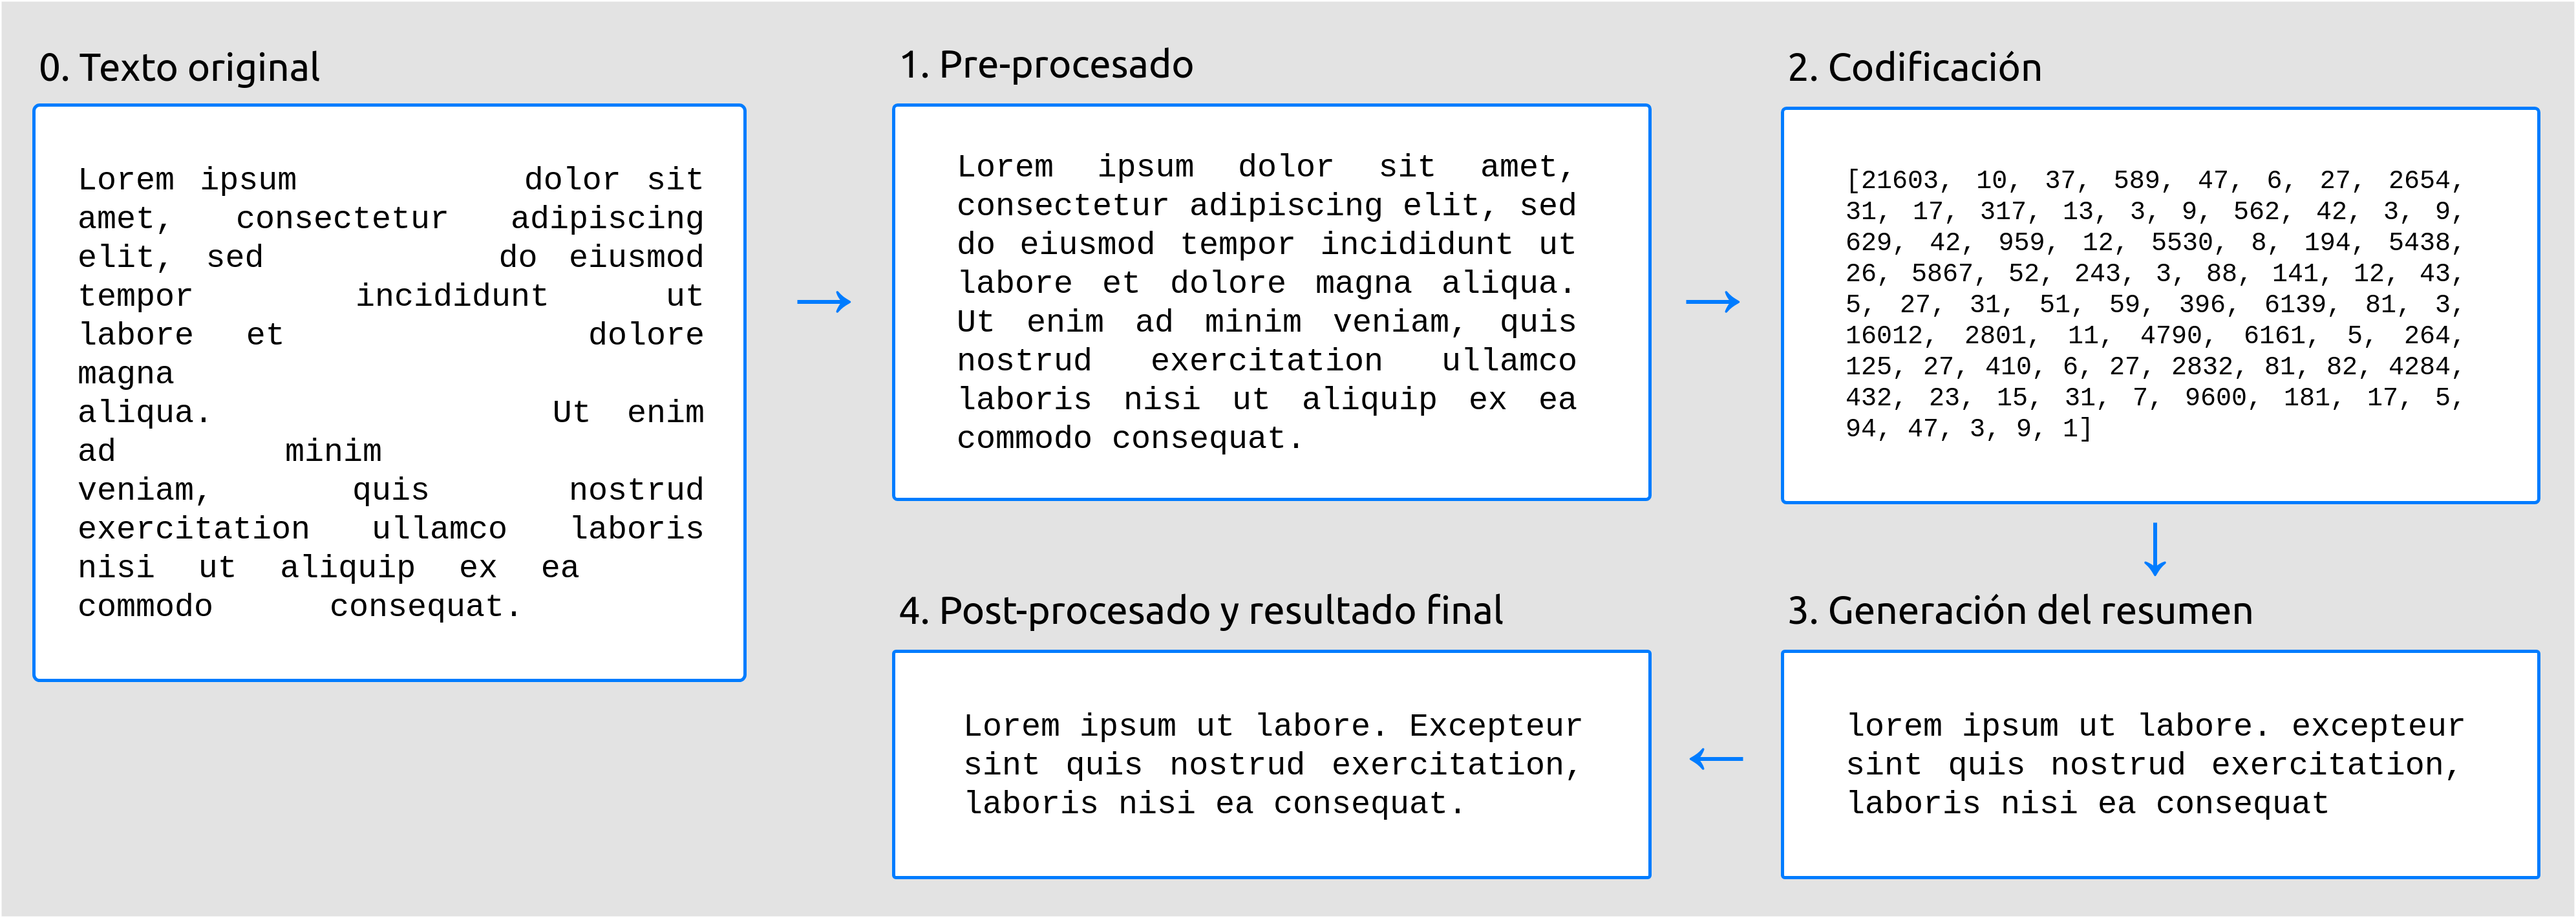
\includegraphics[width=\textwidth]{etapas-resumen}
	\caption{Etapas en la generación de resúmenes.}
	\label{fig:etapas-resumen}
\end{figure}

Veamos en detalle en qué consiste cada una de ellas.

\bigskip
\section{Pre-procesado del texto} \label{sec:preprocesado}

El principal objetivo de esta etapa es adecuar el texto de entrada para que se aproxime lo máximo posible a lo que el modelo espera. Adicionalmente, se separa en texto de entrada en frases. Esta separación puede parecer \emph{a priori} una tarea trivial, pero involucra una serie de dificultades que se detallarán a continuación.

Cabe destacar que, como mencionábamos en la \hyperref[chapter:intro]{Introducción}, los modelos pre-entrenados de los que hacemos uso solo admiten textos en inglés, por lo que algunas de las consideraciones que tomamos en el pre-procesado del texto solo son aplicables a este idioma.

A grandes rasgos, en la etapa de pre-procesado se divide a su vez en los siguientes pasos:

\vspace{-0.4cm}

\begin{itemize}
	\item [\textbullet] Eliminar retornos de carro, tabuladores (\texttt{\textbackslash n}, \texttt{\textbackslash t}) y espacios sobrantes entre palabras (p. ej. \texttt{``I \quad am''} $\rightarrow$ \texttt{``I am''}).
	
	\item [\textbullet] Añadir un espacio al inicio de las frases intermedias (p. ej.: \texttt{``How's it going?Great!''} $\rightarrow$ \texttt{``How's it going? Great!''}. Esto es especialmente relevante en el caso de algunos modelos, como por ejemplo BART \cite{lewis19}, los cuales tienen en cuenta ese espacio inicial para distinguir entre frases iniciales y frases intermedias en la generación de resúmenes\footnote{\, Por el momento, no hacemos uso de este modelo, aunque podría incluirse en el futuro.}.
	
	\item [\textbullet] Establecer un mecanismo que permita llevar a cabo la ya mencionada separación del texto en frases. Esto es importante dado que los modelos tienen un tamaño de entrada máximo. Dos estrategias comunes para eludir esta limitación consisten en (a) truncar el texto de entrada, lo cual puede llevar asociado pérdidas notables de información, o (b) dividir el texto en fragmentos de menor tamaño. En nuestro caso, la primera opción quedó rápidamente descartada ya que los textos que vamos a recibir, por lo general, superarán el tamaño máximo (en caso contrario tendría poco sentido querer generar un resumen). Refiriéndonos, por tanto, a la segunda opción, es frecuente llevar a cabo dicha separación de manera ingenua, únicamente atendiendo al tamaño de entrada máximo. Sin embargo, en nuestro caso decidimos refinar este proceso e implementamos un algoritmo original\footnote{\, Utilizamos el término <<original>> porque no encontramos ningún recurso en el que se tratara este problema, por lo que tuvimos que resolverlo sin apoyos bibliográficos. Esto no quiere decir, sin embargo, que no se hayan implementado estrategias similares en otros problemas diferentes al aquí expuesto.} en el que dicha separación se realiza de tal modo que ninguna frase queda dividida. Para garantizar el éxito de este algoritmo, es fundamental que las frases estén correctamente divididas; el porqué se clarificará en la \hyperref[sec:codificacion]{siguiente sección}, referente a la codificación del texto.
\end{itemize}

A continuación, nos centraremos en el proceso de división del texto en frases. A la hora de llevar a cabo este proceso, debemos tener en cuenta que el texto de entrada podría contener errores ortográficos o gramaticales, por lo que debemos tratar de realizar el mínimo número de suposiciones posibles.

No obstante, la siguiente consideración se nos hace necesaria: el punto (.) indica el final de una frase solo si la siguiente palabra empieza con una letra \emph{y} además mayúscula.

Por ejemplo, en el caso de: \texttt{``Your idea is interesting. However, I would [...].''} se separaría en dos frases, dado que la palabra posterior al punto empieza con una letra mayúscula. Sin embargo: \texttt{``We already mentioned in Section 1.1 that this example shows [...].''} conformaría una única frase, ya que tras el punto no aparece una letra. Procedemos de igual modo en el caso de los signos de interrogación (?) y de exclamación (!). Por ejemplo: \texttt{``She asked \lq How's it going?\rq, and I said \lq Great!\rq.''} se tomará correctamente como una sola frase; tras la interrogación, la siguiente palabra comienza con una letra \emph{minúscula}.
	
Con la suposición anterior, también se agruparían correctamente los puntos suspensivos.

Sin embargo, fallaría en situaciones como: \texttt{``NLP (i.e. Natural Langua}-\texttt{ge Processing) is a subfield of Linguistics, Computer Science, \\ and Artificial Intelligence.''}, en la que la división sería: \texttt{``NLP (i.e.''} por un lado, y \texttt{``Natural Language Processing) is a subfield [...].''}, por otro, ya que \texttt{``Natural''} empieza con mayúscula y aparece tras un punto.

Asimismo, la razón principal por la que no podemos apoyarnos únicamente en reglas predefinidas, reside en las llamadas Entidades Nombradas (\emph{Named Entities}, en inglés), esto es, palabras que hacen referencia a personas, lugares, instituciones, empresas, etc. Existe toda una disciplina dedicada la identificación de este tipo de palabras, conocida como Reconocimiento de Entidades Nombradas (NER, por sus siglas en inglés), y pese a los buenos resultados conseguidos por algunos de los modelos propuestos, se considera un problema lejos de estar resuelto \cite{ner20}.

En nuestro caso emplearemos un modelo pre-entrenado para solucionar, al menos en parte, el problema de las Entidades Nombradas. Este modelo también solventa situaciones como la descrita anteriormente, en las que las reglas escritas a mano se quedan cortas. En el capítulo de \hyperref[chapter:tecnicas]{Técnicas y Herramientas}, hablaremos de dicho modelo y de la implementación concreta en código de los procedimientos expuestos anteriormente.

\bigskip

\section{Codificación del texto} \label{sec:codificacion}

En esta etapa, se lleva a cabo lo que se conoce en inglés como \emph{word embedding}\footnote{\, En el presente documento, hemos traducido este término como <<codificación del texto>>.}. Los modelos de IA trabajan, por lo general, con representaciones númericas. Por ello, las técnicas de \emph{word embedding} se centran en vincular texto (bien sea palabras, frases, etc.), con vectores de números reales \cite{manning19}. Esto hace posible aplicar a la generación de texto arquitecturas comunes dentro de la IA (y especialmente, del \emph{Deep Learning}), como por ejemplo las Redes Neuronales Convolucionales (CNN) \cite{hou20}.

Esta idea, conceptualmente sencilla, encierra una gran complejidad, dado que los vectores generados deben retener la máxima información posible del texto original, incluyendo aspectos semánticos y gramaticales. Por poner un ejemplo, los vectores correspondientes a las palabras <<profesor>> y <<alumno>>, deben preservar cierta relación entre ambos, y a su vez con la palabra <<educación>> o <<escuela>>. Además, su vínculo con las palabras <<enseñar>> o <<aprender>> será ligeramente distinto, dado que en este caso se trata de una categoría gramatical diferente (verbos, en vez de sustantivos). A través de este ejemplo, podemos comprender que se trata de un proceso complejo.

Dado que los modelos pre-entrenados se encargan de realizar esta codificación por nosotros, no entraremos en más detalle en los algoritmos concretos empleados, dado que consideramos que queda fuera del alcance de este trabajo\footnote{\, En cualquier caso, el lector curioso puede explorar los algoritmos más populares de codificación, los cuales, ordenados cronológicamente, son: word2vec \cite{word2vec1, word2vec2}, GloVe \cite{glove14}, y más recientemente, ELMo \cite{elmo18} y BERT \cite{bert18}.}.

Lo que sí hemos tenido que implementar en esta etapa, ha sido la división del texto en fragmentos a fin de no superar el tamaño máximo de entrada del modelo.

De este modo, podremos realizar resúmenes de textos arbitrariamente largos, a través de los siguientes pasos:

\vspace{-\baselineskip}
\begin{enumerate}
	\tightlist
	\item Dividimos el texto en fragmentos.
	\item Generamos un resumen de cada fragmento.
	\item Concatenamos los resúmenes generados.
\end{enumerate}
\vspace{-0.3cm}

Anteriormente, habíamos mencionado el término \emph{token}. Este concepto se puede traducir al español como <<símbolo>>. En nuestro caso concreto, un \emph{token} se corresponde con el vector numérico asociado a una palabra al realizar la codificación. Más concretamente, en modelos más actuales, como el modelo T5 \cite{raffel19}, los \emph{tókenes} pueden referirse a palabras completas o a \emph{fragmentos} de las mismas.

Por lo general, las palabras que aparecen en el vocabulario con el que ha sido entrenado el modelo van a generar un único \emph{token}. Sin embargo, las palabras desconocidas, se descompondrán en varios \emph{tókenes}. Lo mismo sucede con palabras compuestas o formadas a partir de prefijación o sufijación. En la \hyperref[fig:t5-tokenizer]{siguiente figura}, podemos ver un ejemplo de ello:

\begin{figure}[h]
	\centering
	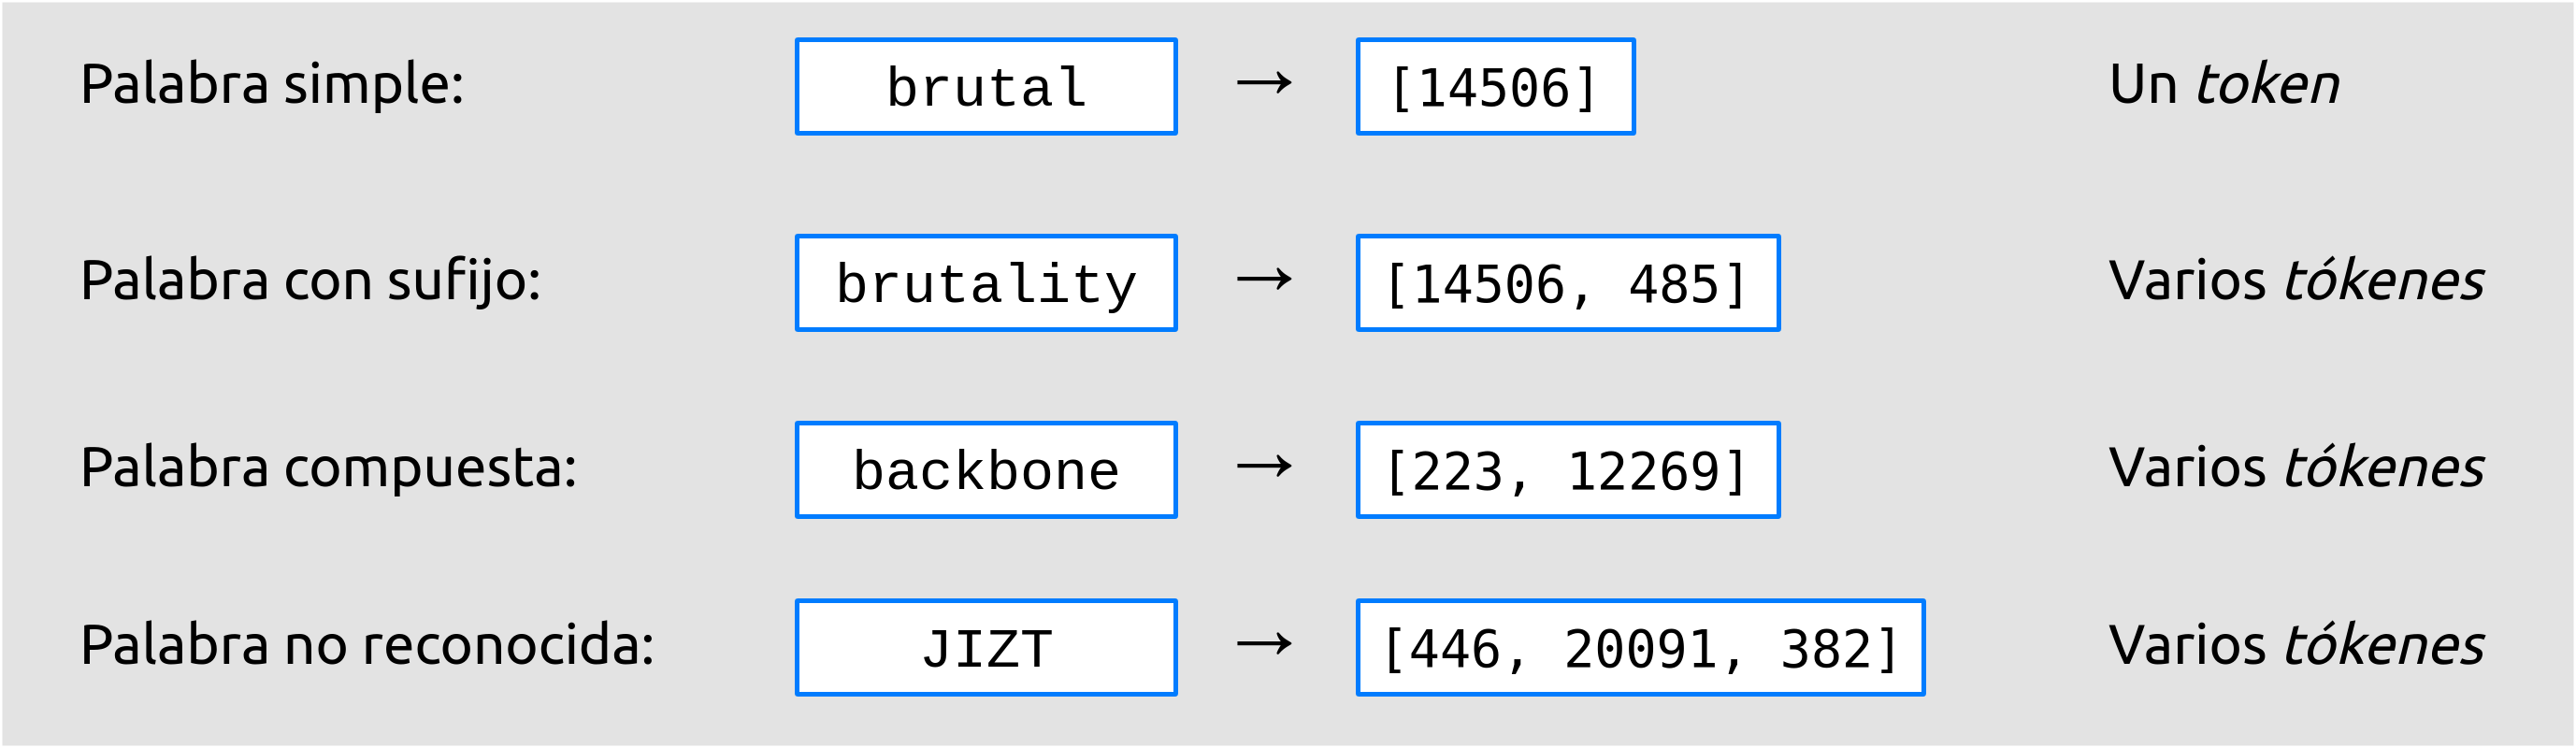
\includegraphics[width=1.035\textwidth]{t5-tokenizer}
	\caption{Ejemplo de \emph{tokenización} con el modelo T5.}
	\label{fig:t5-tokenizer}
\end{figure}

En el anterior ejemplo, si decodificamos los \emph{tókenes} correspondientes a la palabra \texttt{``backcone''}, esto es, \texttt{[223, 12269]}, obtenemos los fragmentos \texttt{``back''}, y \texttt{``bone''}, respectivamente.

La idea detrás de esta fragmentación se basa en la composición, uno de los mecanismos morfológicos de formación de palabras más frecuentes \cite{cetnarowska05} en muchos idiomas, como el inglés, español o alemán. Por tanto, presupone que dividiendo las palabras desconocidas en fragmentos menores, podemos facilitar la comprensión de las mismas. Naturalmente, habrá casos en los que esta idea falle; por ejemplo, en la figura anterior, la palabra \texttt{``JIZT''} se descompone en \texttt{``J''}, \texttt{``IZ''}, \texttt{``T''}, lo cual no parece hacerla mucho más comprensible.

Una vez explicado el concepto de \emph{token}, volvamos al problema ya mencionado con anterioridad: algunos modelos de generación de texto (entre ellos, el T5) admiten un tamaño de entrada máximo, determinado en función del número de \emph{tókens}. Debido a que la unidad de medida es el número de \emph{tókenes}, y no el número de palabras, o de caracteres, debemos tener en cuenta algunos detalles, entre ellos el hecho de que los modelos generan \emph{tókenes} especiales para marcar el inicio y/o el final de la secuencia de entrada.

El modelo T5 (el cual como mencionábamos anteriormente, es el único modelo que utilizamos por ahora), genera un único \emph{token} de finalización de secuencia (EOS, \emph{end-of-sequence}), que se coloca siempre al final del texto de entrada, una vez codificado, y en el caso de de este modelo siempre tiene el \emph{id} 1. En la \hyperref[fig:t5-eos-ejemplo]{siguiente figura} podemos ver un ejemplo con un texto de entrada:

\begin{figure}[h]
	\centering
	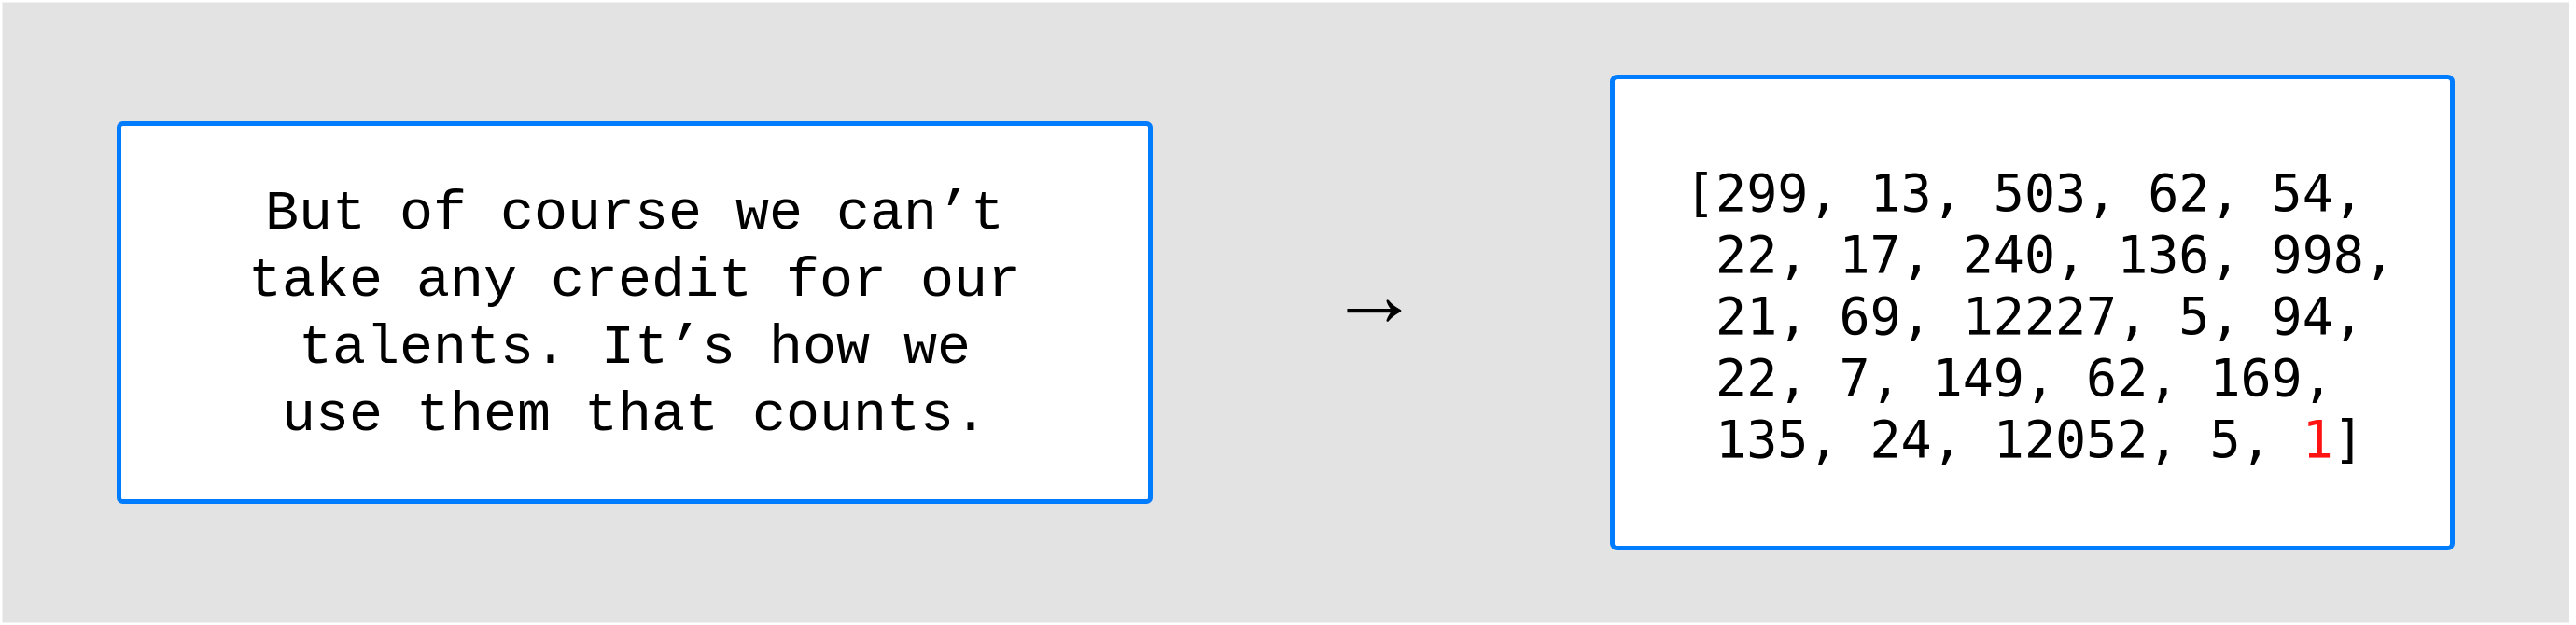
\includegraphics[width=\textwidth]{t5-eos-ejemplo}
	\caption[Ejempo de codificación del texto.]{Pasaje del libro \emph{A Wrinkle in Time}. El \emph{tóken} EOS se ha marcado en rojo.}
	\label{fig:t5-eos-ejemplo}
\end{figure}

Como podemos ver, el \emph{tóken} EOS aparece una única vez por cada texto de entrada, y es independiente de las palabras o frases que este contiene.

Otro aspecto a tener en cuenta, reside en que este modelo no solo es capaz de generar resúmenes, si no que puede ser empleado para otras tareas como la traducción, respuesta de preguntas \cite{raffel19}, etc. Para indicarle cuál de estas es la tarea que queremos que desempeñe, curiosamente se lo tenemos que indicar tal y cómo lo haríamos en la vida real; en nuestro caso, simplemente precedemos el texto a resumir con la orden <<resume>> (<<\emph{summarize}>>). Por poner otro ejemplo, si quisiéramos traducir del alemán al español, le señalaríamos: <<traduce de alemán a español>> seguido de nuestro texto (<<\emph{summarize German to Spanish}>>).

Por consiguiente, este prefijo deberá aparecer al principio de cada una de las subdivisiones generadas y, del mismo modo, deberemos tenerlo en cuenta a la hora de calcular el número de \emph{tókenes} de las mismas.

Con las anteriores consideraciones en mente, el objetivo principal será llevar a cabo la división del texto de entrada de forma que el número de \emph{tókenes} varíe lo mínimo posible entre las diferentes subdivisiones, y todo ello sin partir ninguna frase.

Esta es una tarea más compleja de lo que puede parecer. En nuestro caso, hemos propuesto un \hyperref[alg:division-codificacion]{algoritmo} que emplea una estrategia voraz para llevar a cabo una primera división del texto; posteriormente procede al \emph{balanceo} de las subdivisiones generadas en el paso anterior, de forma que el número de \emph{tókenes} en cada subdivisión sea lo más parecido posible. Y esto, evidentemente, sin superar el máximo tamaño de entrada del modelo en ninguna de las subdivisiones.

\newcommand\CONDITION[2]%
{\begin{tabular}[t]{@{}l@{}}
		#1 #2
 \end{tabular}%
}
\algdef{SE}[WHILE]{While}{EndWhile}[1]%
{\algorithmicwhile\ \CONDITION{#1}{\ \algorithmicdo}}%
{\algorithmicend\ \algorithmicwhile}
\algdef{SE}[FOR]{For}{EndFor}[1]%
{\algorithmicfor\ \CONDITION{#1}{\ \algorithmicdo}}%
{\algorithmicend\ \algorithmicfor}
\algdef{S}[FOR]{ForAll}[1]%
{\algorithmicforall\ \CONDITION{#1}{\ \algorithmicdo}}
\algdef{SE}[REPEAT]{Repeat}{Until}{\algorithmicrepeat}[1]%
{\algorithmicuntil\ \CONDITION{#1}{}}
\algdef{SE}[IF]{If}{EndIf}[1]%
{\algorithmicif\ \CONDITION{#1}{\ \algorithmicthen}}%
{\algorithmicend\ \algorithmicif}%
\algdef{C}[IF]{IF}{ElsIf}[1]%
{\algorithmicelse\ \algorithmicif\ \CONDITION{#1}{\ \algorithmicthen}}
\begin{algorithm}
	\caption{División y codificación del texto.}\label{alg:division-codificacion}
	\begin{algorithmic}[1]
		\Procedure{CodificaciónConDivisión}{$texto, prefijo$}
		\State $frases \gets \text{dividirEnFrases(\textit{texto})}$
		\State $frasesCodif \gets [\,]$ \Comment{Frases codificadas}
		\State $prefijoCodif \gets \text{codifica(\textit{prefijo})}$
		\State $EOSCodif \gets \text{codifica(\textit{EOS})}$ \Comment{Token EOS codificado}
		\State $subdivsCodif \gets [\,]$ \Comment{Subdivisiones codificadas}
		
		\For{$\textit{fr} \enspace\text{\textbf{in}}\; \textit{frases}$}
			\State $frasesCodif \gets \text{codifica(\textit{fr})}[:-1]$ \Comment{Excluir EOS}
		\EndFor
		
		\State $ptosCorte \gets \text{divideVoraz(\textit{frasesCodif}, \textit{prefijoCodif})}$
		
		\State $ptosCorte \gets \text{balanceaSubdivs(\textit{ptosCorte})}$

		\For{$i \gets 0, \text{len(\textit{ptosCorte}) - 1}$}
			\State $frasesSubvid \gets frasesCodif[ptosCorte[i]:ptosCorte[i+1]]$ \Comment{Frases en subdiv.}
			\State $subdivsCodif[i] \gets \text{concatena(\textit{prefijoCodif}, \textit{frasesSubdiv}, \textit{EOSCodif})}$
		\EndFor
		\State \textbf{return} $subdivsCodif$
		\State \hspace{-0.5cm}\textbf{end procedure}
		\EndProcedure
	\end{algorithmic}
\end{algorithm}

Este algoritmo devuelve las subdivisiones en las que se ha separado el texto, ya codificadas. Por tanto, $subdivsCofif$ tendrá la siguiente forma:

\vspace{-0.5cm}

\[ [[23, 34, 543, 45, ..., 1], [23, 32. 401, 11, ..., 1], [23, 74. 25, 204, ..., 1], ...] \]

Es decir, cada una de las listas contenidas en $subdivsCodif$ contiene los \emph{tókenes} correspondientes a dicha subdivisión, con el prefijo (23) y el \emph{token} EOS (1) añadidos.
	
La lógica detrás de la función $divideVoraz$ es la siguiente:

\begin{algorithm}
	\caption{División voraz del texto.}\label{alg:divide-voraz}
	\begin{algorithmic}[1]
		\Procedure{DivideVoraz}{$frasesCodif, prefijoCodif$}
		\State $ptosCorte \gets [0]$
		\State $lenSubdiv = \text{len(\textit{prefijoCodif})} + \text{len(\textit{frasesCodif}[0])} + 1$ \Comment Contar prefijo y EOS
		\For{$i \gets 0, \text{len(\textit{frasesCodif}) - 1}$}
			\State $lenSubdiv = lenSubdiv + \text{len(\textit{frasesCodif}[i])}$
			\If{lenSubdiv > \, model.maxLength}
				\State $ptosCorte.\text{añadir(\textit{i})}$
				\State $lenSubdiv = \text{len(\textit{prefijoCodif})} + \text{len(\textit{frasesCodif}[i])} + 1$
			\EndIf
		\EndFor
		\State $ptosCorte.\text{añadir(len(\textit{frasesCodif}))}$
		\State \textbf{return} $ptosCorte$
		\State \hspace{-0.5cm}\textbf{end procedure}
		\EndProcedure
	\end{algorithmic}
\end{algorithm}

Es decir, $ptosCorte$ será una lista que indique los índices que delimitan cada subdivisión, por ejemplo:

\vspace{-0.5cm}

\[ [0, 45, 91, 130, 179, 190] \]

En este caso, la primera subdivisión iría desde la frase 0 hasta la 45, la segunda subdivisión de la 46 a la 91, la tercera de la 92 a la 130, y así sucesivamente.

Como podemos ver en el ejemplo, el número de \emph{tókenes} por subdivisión está en torno a los 45, menos en la última subdivisión que solo contiene 10 \emph{tókenes} ($190-180$). Debido a la propia naturaleza del algoritmo voraz, será siempre la última subdivisión la que pueda contener un número de \emph{tókenes} muy por debajo de la media, lo que puede causar que el resumen de está última subdivisión sea demasiado corto (o incluso sea la cadena vacía). Para evitar esto, balanceamos las subdivisiones, de forma que el número de \emph{tókenes} en cada una de ellas esté equilibrado.


\algdef{SE}[DOWHILE]{Do}{DoWhile}{\algorithmicdo}[1]{\algorithmicwhile\ #1}%
\begin{algorithm}
	\caption{Balanceo de las subdivisiones.}\label{alg:balancea-subdivs}
	\begin{algorithmic}[1]
		\Procedure{BalanceaSubdivs}{$ptosCorte$}
		\State $ptosCorteBalan \gets ptosCorte$ \Comment{Puntos de corte balanceados}

		\Do
			\State $ptosCorteBalanOld \gets ptosCorteBalan$
			\For{$i \gets \text{len(\textit{ptosCorteBalan})} - 1, 1, step: - 1$} \Comment{Empezar por última subdiv.}
			\State $\textit{diffLen} \gets \text{lenSubdiv(\textit{i} -1)} - \text{lenSubdiv(\textit{i})}$ \Comment{Diferencia en n. de \emph{tókenes}}
			\While{$\textit{diffLen} > 0$}
				\State $últimaFrase \gets \text{getÚltimaFrase(getSubdiv(\textit{i}-1))}$
				
				\If{$\text{getSubdiv(\textit{i}) + len(\textit{últimaFrase}) <= model.maxLength} \enspace \wedge$ \\ \hspace{0.5cm} $\text{len(\textit{últimaFrase}) <= \textit{diffLen}}$}
				\State $\text{mueveÚltimaFrase(getSubdiv(\textit{i}-1), getSubdiv(\textit{i}))}$
				\State $ptosCorteBalan[i-1] \gets ptosCorteBalan[i-1] - 1$
				\Else \\ \hspace{2.42cm}\textbf{\emph{break}}
				\EndIf
			\EndWhile
			\EndFor
		\DoWhile{$ptosCorteBalan \not = ptosCorteBalanOld$}
		\State \textbf{return} $ptosCorte$
		\State \hspace{-0.5cm}\textbf{end procedure}
		\EndProcedure
	\end{algorithmic}
\end{algorithm}

En esencia, lo que este último algoritmo hace es comparar la diferencia en número de \emph{tókenes} entre subdivisiones consecutivas, empezando por el final, de forma que primero se compara la penúltima con la última subdivisión, después la antepenúltima con la penúltima, y así sucesivamente. Si es necesario, va moviendo frases completas desde una subdivisión a la siguiente, por ejemplo, desde la penúltima a la última subdivisión. Este algoritmo tiene una complejidad en el peor de los casos de $O(n^3)$, siendo $n$ el número de subdivisiones.

Podemos visualizarlo gráficamente con un ejemplo muy simple:

\begin{figure}[h]
	\centering
	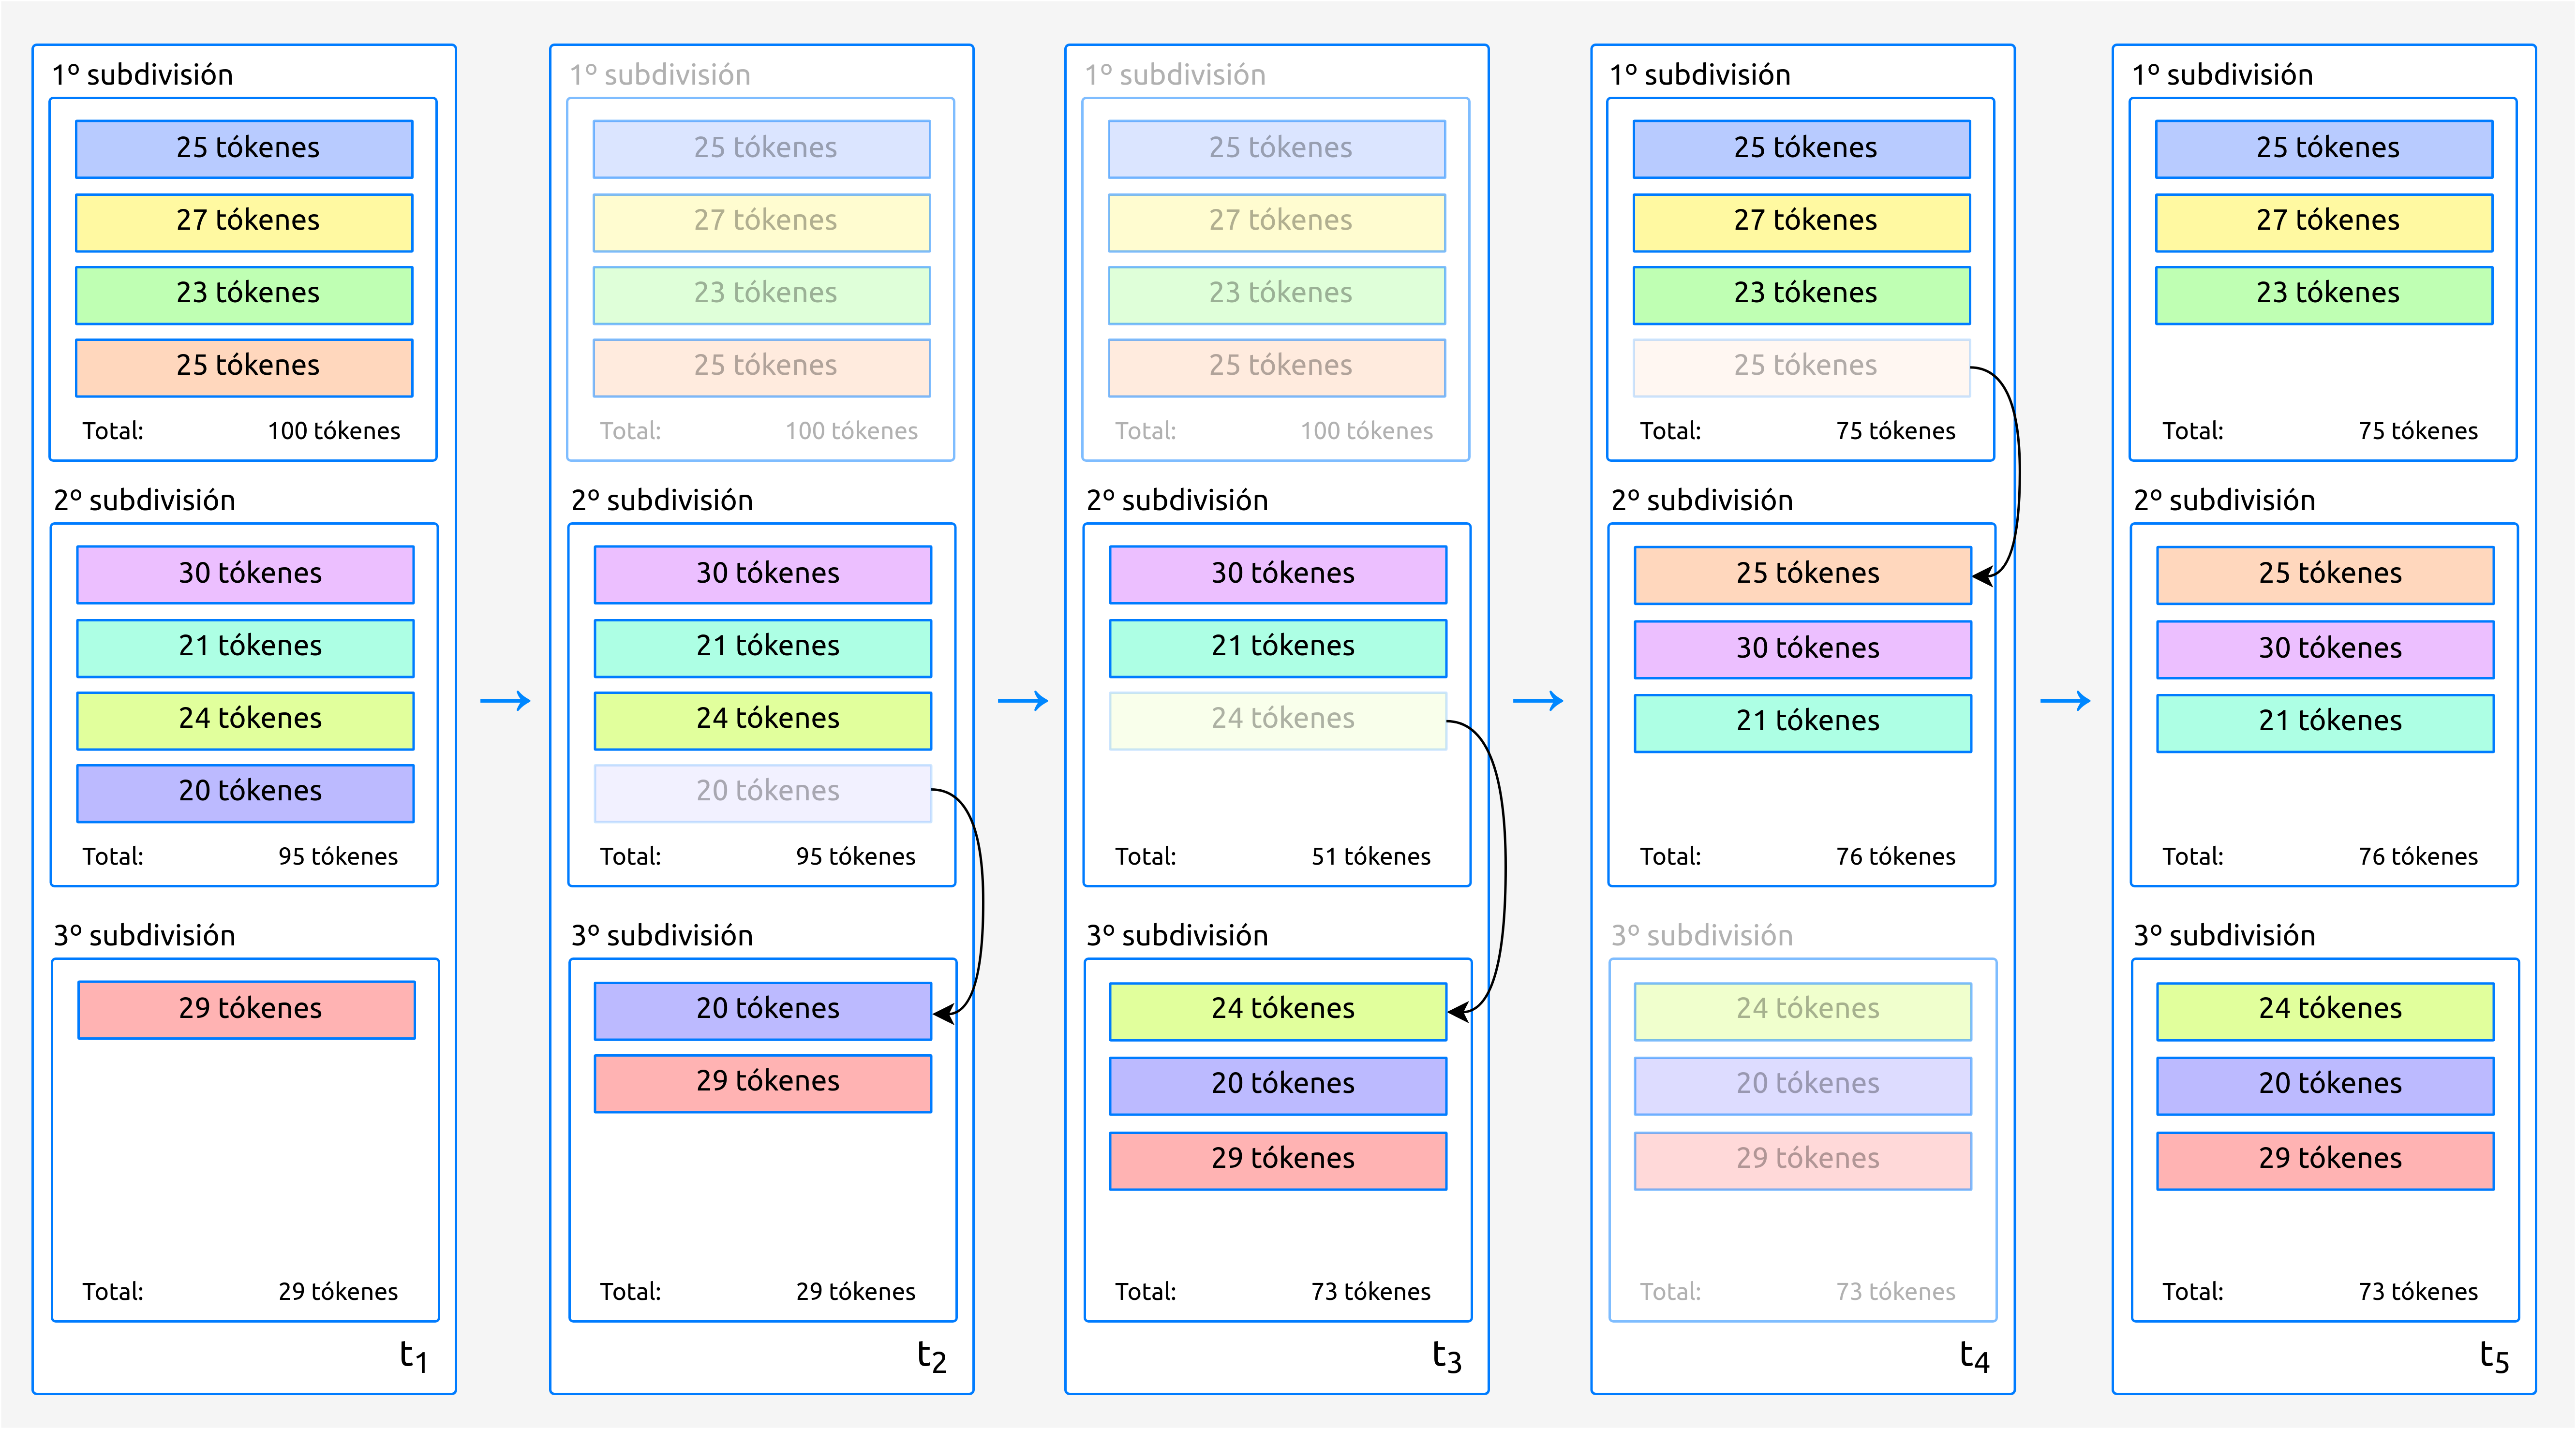
\includegraphics[width=\textwidth]{algoritmo-balanceo}
	\caption[Ejemplo gráfico del algoritmo de balanceo.]{Ejemplo gráfico del algoritmo de balanceo. Las desviación estándar del número de \emph{tókenes} de cada frase en $t_1$ es $\sigma_1 = 39.63$ y en $t_5$, acaba siendo $\sigma_5 = 1.53$.}
	\label{fig:algoritmo-balanceo}
\end{figure}

\newpage

\section{Generación del resumen} \label{sec:resumen}

Una vez codificado y dividido el texto apropiadamente, generamos los resúmenes parciales para posteriormente unirlos, dando lugar a un único resumen del texto completo.

En la \autoref{fig:proceso-resumen}, podemos ver los pasos llevados a cabo tanto en la anterior etapa, la codificación y división del texto, como en esta, la generación del resumen.

\begin{figure}[h]
	\centering
	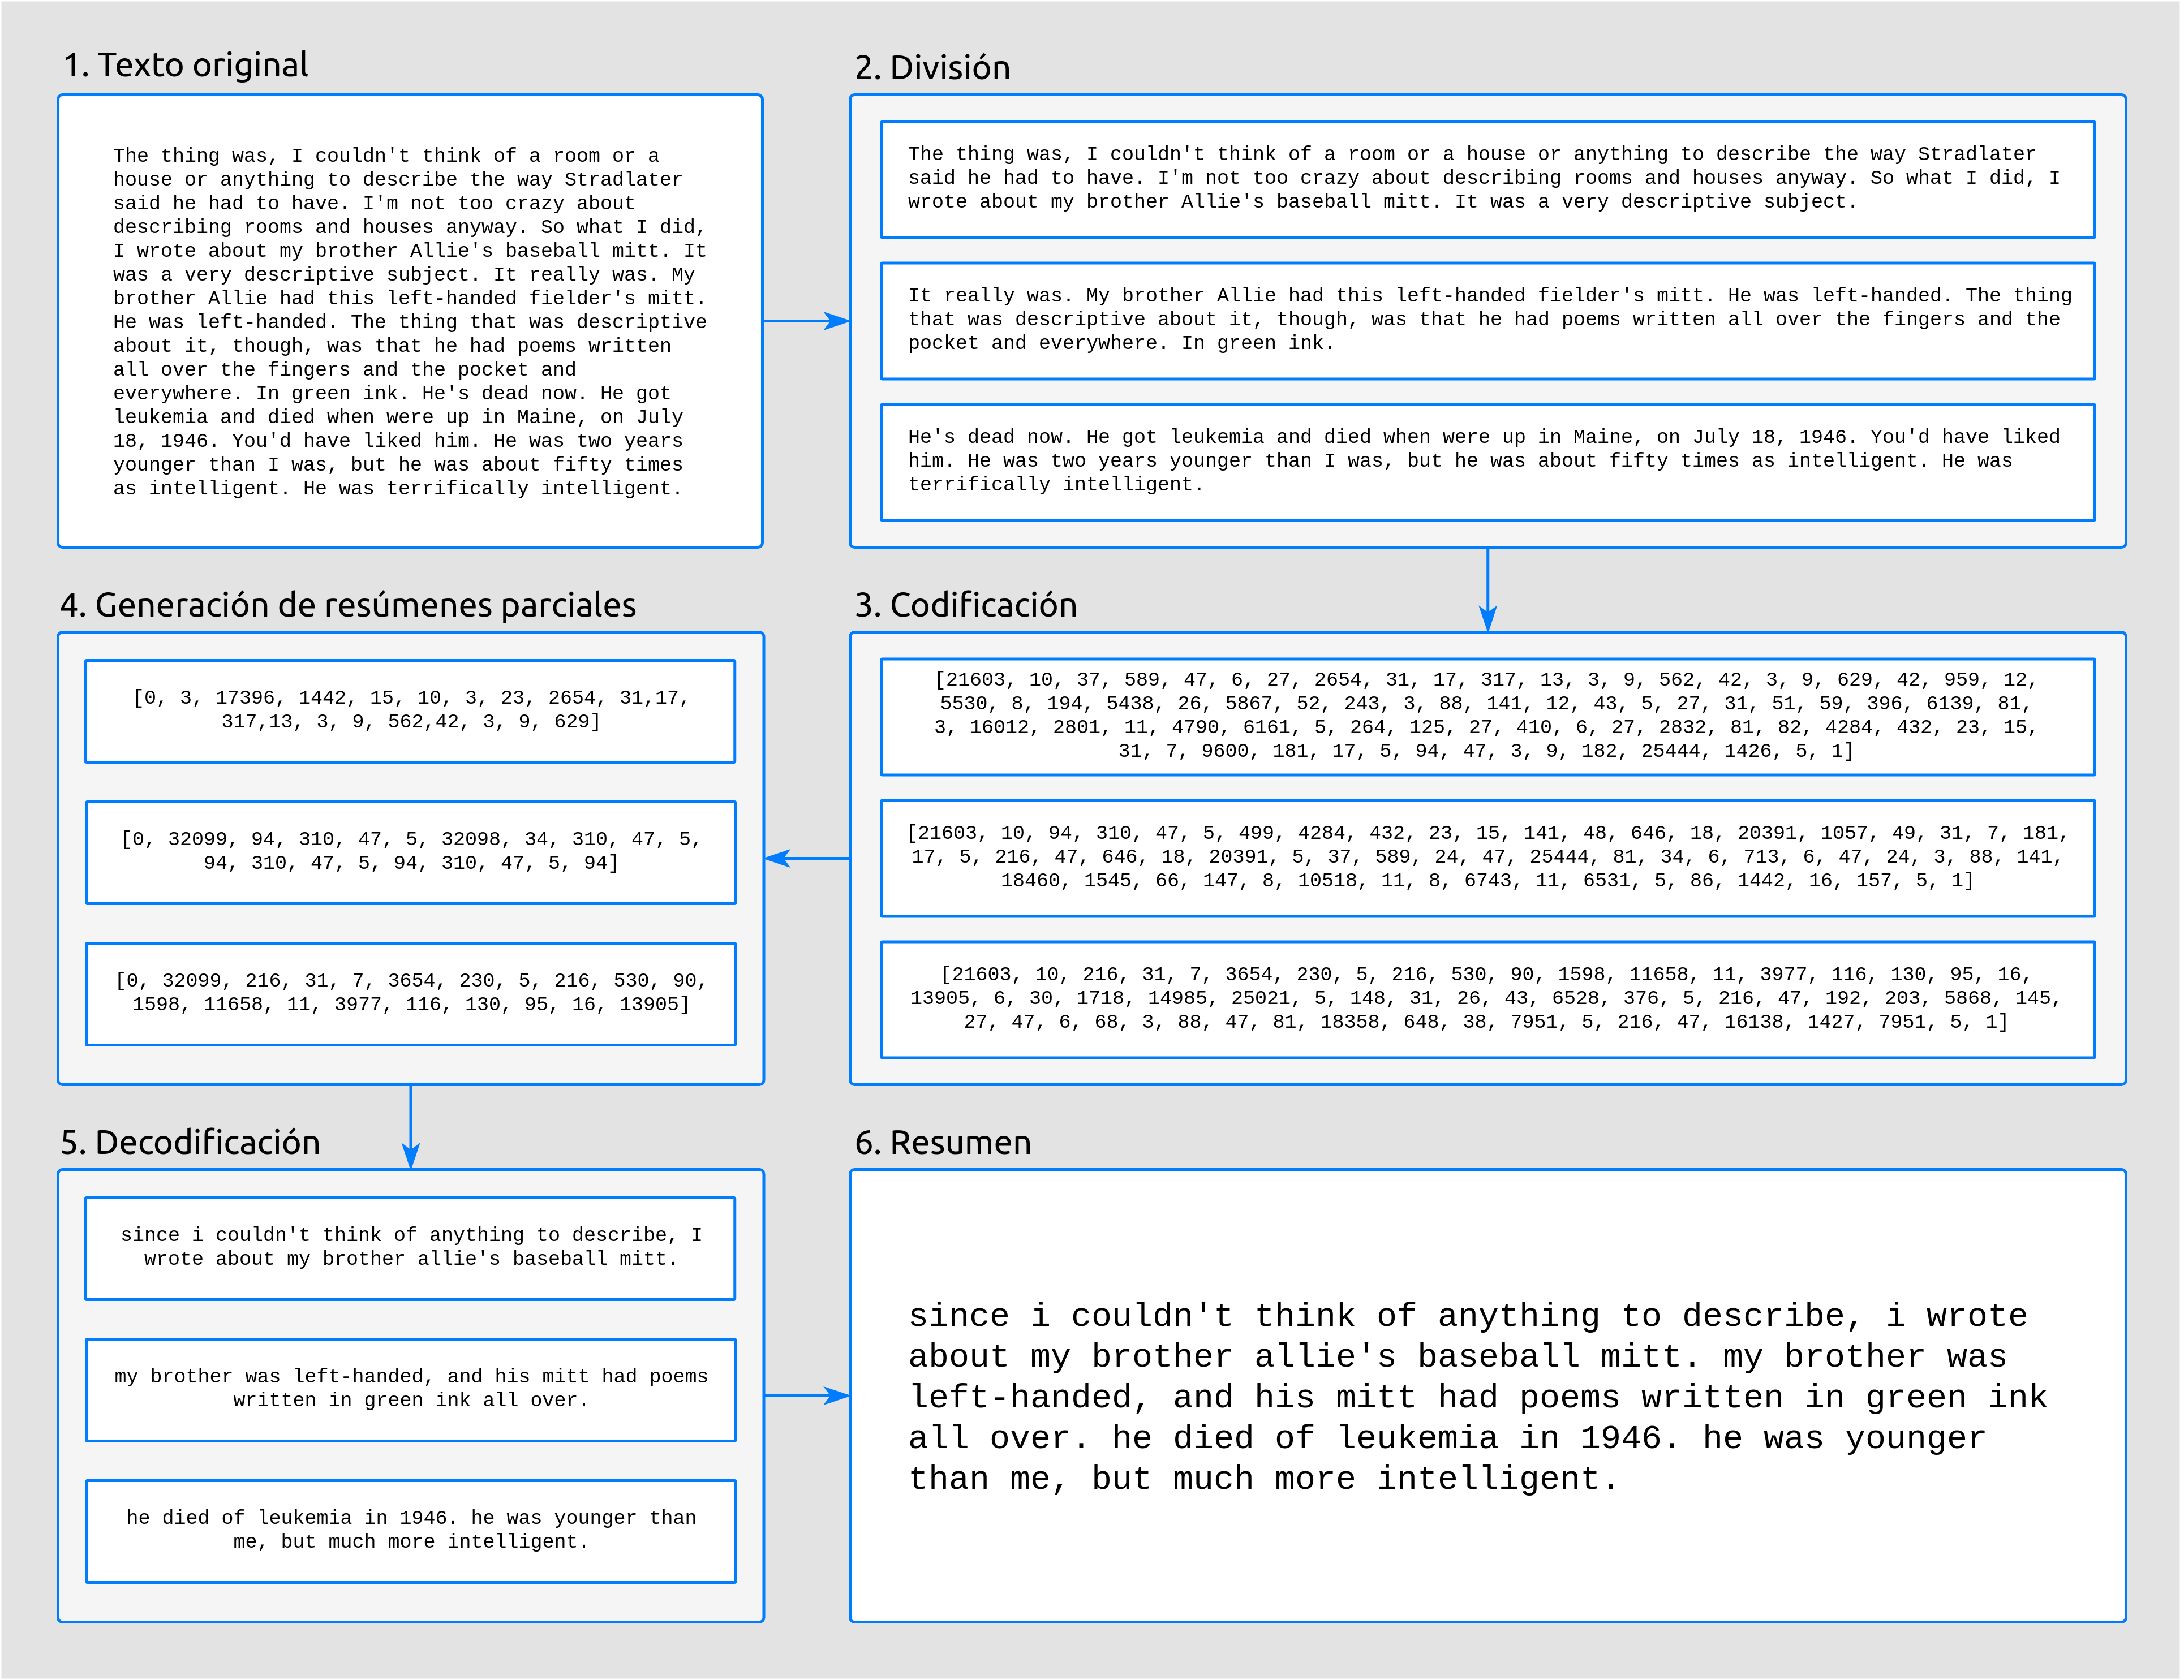
\includegraphics[width=\textwidth]{t5-proceso-resumen}
	\caption[Proceso de generación de resúmenes.]{Proceso de generación de resúmenes, ilustrado con un fragmento del libro \emph{The Catcher in the Rye}.}
	\label{fig:proceso-resumen}	
\end{figure}

Como podemos apreciar en la anterior figura, el modelo generador de resúmenes toma el texto codificado, y devuelve una versión reducida del mismo, también codificado. Por ello, antes de poder unir y devolver el resumen generado, debemos realizar un paso de \emph{decodificación}, que realiza el proceso contrario a la \emph{codificación}, como veíamos en la \hyperref[sec:codificacion]{anterior sección}. Algo con lo que tendremos que lidiar en la siguiente etapa, el post-procesado, será corregir el resumen generado para que se ajuste a las reglas ortográficas vigentes, en especial en lo relativo al uso de mayúsculas.

La ventaja de utilizar modelos pre-entrenados es clara: estos modelos son para nosotros cajas negras, a las que solo tenemos que encargarnos de proporcionarles la entrada en el formato concreto que esperan.

Cabe destacar que, el hecho de realizar la división del texto de esta manera, sin atender a aspectos semánticos, podría resultar en que en frases estrechamente relacionadas acabaran en distintas subdivisiones. Por ejemplo, en la \autoref{fig:proceso-resumen}, la frase final de uno de las subdivisiones es: \emph{<<It was a very descriptive subject>>} (<<Era un tema muy descriptivo>>), a la cual le sigue, ya en la siguiente subdivisión: \emph{<<It really was>>} (<<De veras que lo era>>), aludiendo a la anterior frase.

Estos casos son difíciles de resolver. Una posible idea sería tratar de determinar si una frase está relacionada con la anterior, quizás mediante el uso de otro modelo, y de ser así, tratar de mantenerlas en una misma subdivisión, a fin de que el resumen final mantenga la máxima cohesión y coherencia posibles. Esto incrementaría, no obstante, los tiempos de generación de resúmenes. Por ahora, creemos que los resultados obtenidos son lo suficientemente buenos.

\bigskip
\subsubsection{Modelo empleado para la generación de resúmenes: T5}

Come hemos mencionado previamente, JIZT hace uso del modelo T5 \cite{raffel19} de Google. Este modelo fue introducido en el artículo \emph{Exploring the Limits of Transfer Learning with a Unified Text-to-Text Transformer}, presentado en 2019. En él, Colin Raffel \emph{et al.} estudian las ventajas de la técnica del aprendizaje por transferencia (\emph{transfer learning}) al campo del Procesamiento del Lenguaje Natural (NLP).

Tradicionalmente, cada nuevo modelo se entrenaba desde cero. Esto ha cambiado con la inclusión del aprendizaje por transferencia; actualmente, la tendencia es emplear modelos pre-entrenados como punto de partida para la construcción de nuevos modelos.

Las tres principales ventajas del empleo del aprendizaje por transferencia son \cite{sarkar18}:

\vspace*{-\baselineskip}
\begin{itemize}
	\item [\textbullet] Mejora del rendimiento de partida. El hecho de comenzar con un modelo pre-entrenado en vez de un modelo ignorante (\emph{ignorant learner}), proporciona un rendimiento base desde el primer momento.
	
	\item [\textbullet] Disminución del tiempo de desarrollo del modelo, consecuencia del punto anterior.
	
	\item [\textbullet] Mejora del rendimiento final. Esta mejora ha sido estudiada tanto en el caso del NLP \cite{kumar21}, como de otros ámbitos, como la visión artificial \cite{ali21}, o el campo de la medicina \cite{liu21}.
\end{itemize}

La principal novedad de este artículo se encuentra en su propuesta de tratar todos los problemas de procesamiento de texto como problemas texto a texto (\emph{text-to-text}), es decir, tomar un texto como entrada, y producir un nuevo texto como salida. Esto permite crear un modelo general, al que han bautizado como T5, capaz de llevar a cabo diversas tareas de NLP, como muestra el siguiente diagrama:

\bigskip


\begin{figure}[h]
	\centering
	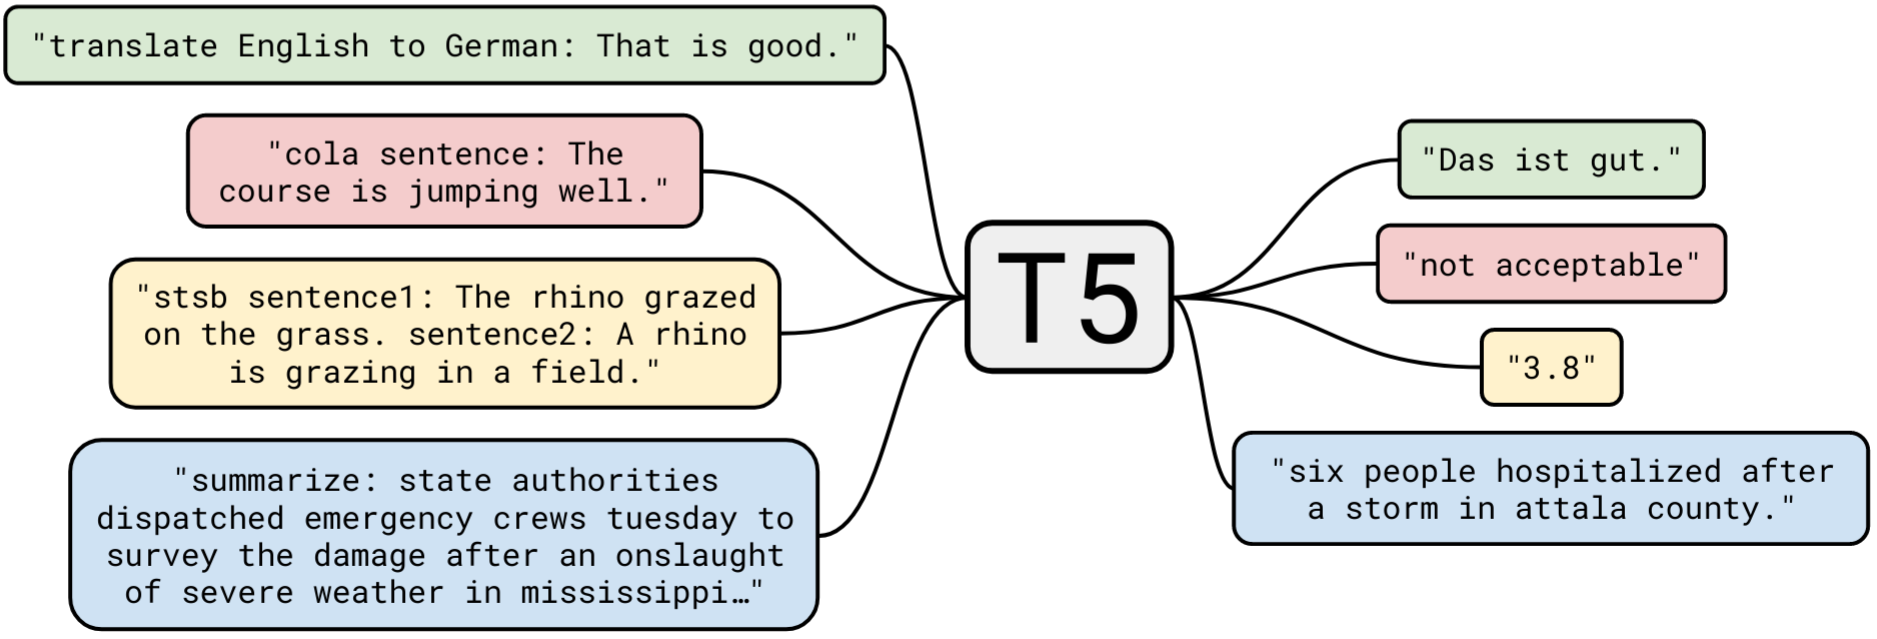
\includegraphics[width=\textwidth]{t5-paper}
	\caption[Ejemplo del modelo T5 de Google.]{El \emph{framework} texto a texto permite emplear el mismo modelo, con los mismos hiperparámetros, función de pérdida, etc., para aplicarlo a diversas tareas de NLP \cite{raffel19}.}
\end{figure}


En cualquier caso, se puede realizar un ajuste fino del modelo para una de las tareas, a fin de mejorar su rendimiento en dicha tarea específica.

Las posibilidades que este modelo nos ofrece son muy interesantes, dado que en un futuro, nuestro proyecto podría incluir otras tareas de Procesamiento de Lenguaje Natural, haciendo uso de un solo modelo.


\bigskip
\subsubsection{Principales estrategias de generación de resúmenes} \label{subsec:estrategias-gen}

JIZT permite al usuario avanzado configurar de manera precisa los parámetros con los que se genera el resumen. En este apartado, exploraremos las diferentes técnicas con las que se pueden generar resúmenes.

La generación de lenguaje, en general, se basa en la auto-regresión, la cual parte del supuesto de que la distribución de probabilidad de una secuencia de palabras puede descomponerse en el producto de las distribuciones de probabilidades  condicionales de las palabras sucesivas \cite{platen20}. Expresado matemáticamente:

\[ P(w_{1:t} | W_0) = \prod_{t=1}^{T} P(w_t | w_{1:t-1}, W_0), \; siendo \enspace w_{1:0} = \emptyset \]

donde $W_0$ es la secuencia inicial de \emph{contexto}. En nuestro caso, esa secuencia inicial va a ser el propio texto de entrada. La longitud de $T$ no se puede conocer de antemano, dado que se corresponde con el momento $t = T$ en el que el modelo genera el \emph{token} de finalización de secuencia ()EOS), mencionado anteriormente.

Una vez introducido el concepto de auto-regresión, podemos explicar brevemente las cinco	 principales estrategias de generación de lenguaje, las cuales se pueden aplicar todas ellas a la generación de resúmenes: búsqueda voraz, \emph{beam search}, muestreo, muestreo \emph{top-k}, y muestreo \emph{top-p}.

\bigskip
\noindent
\textbf{Búsqueda voraz}

La búsqueda voraz, en cada paso, simplemente selecciona la palabra con mayor probabilidad de ser la siguiente, es decir, $ w_t = argmax_w P(w|w_{t-1}) $ para cada paso \emph{t}.

\begin{figure}[h]
	\centering
	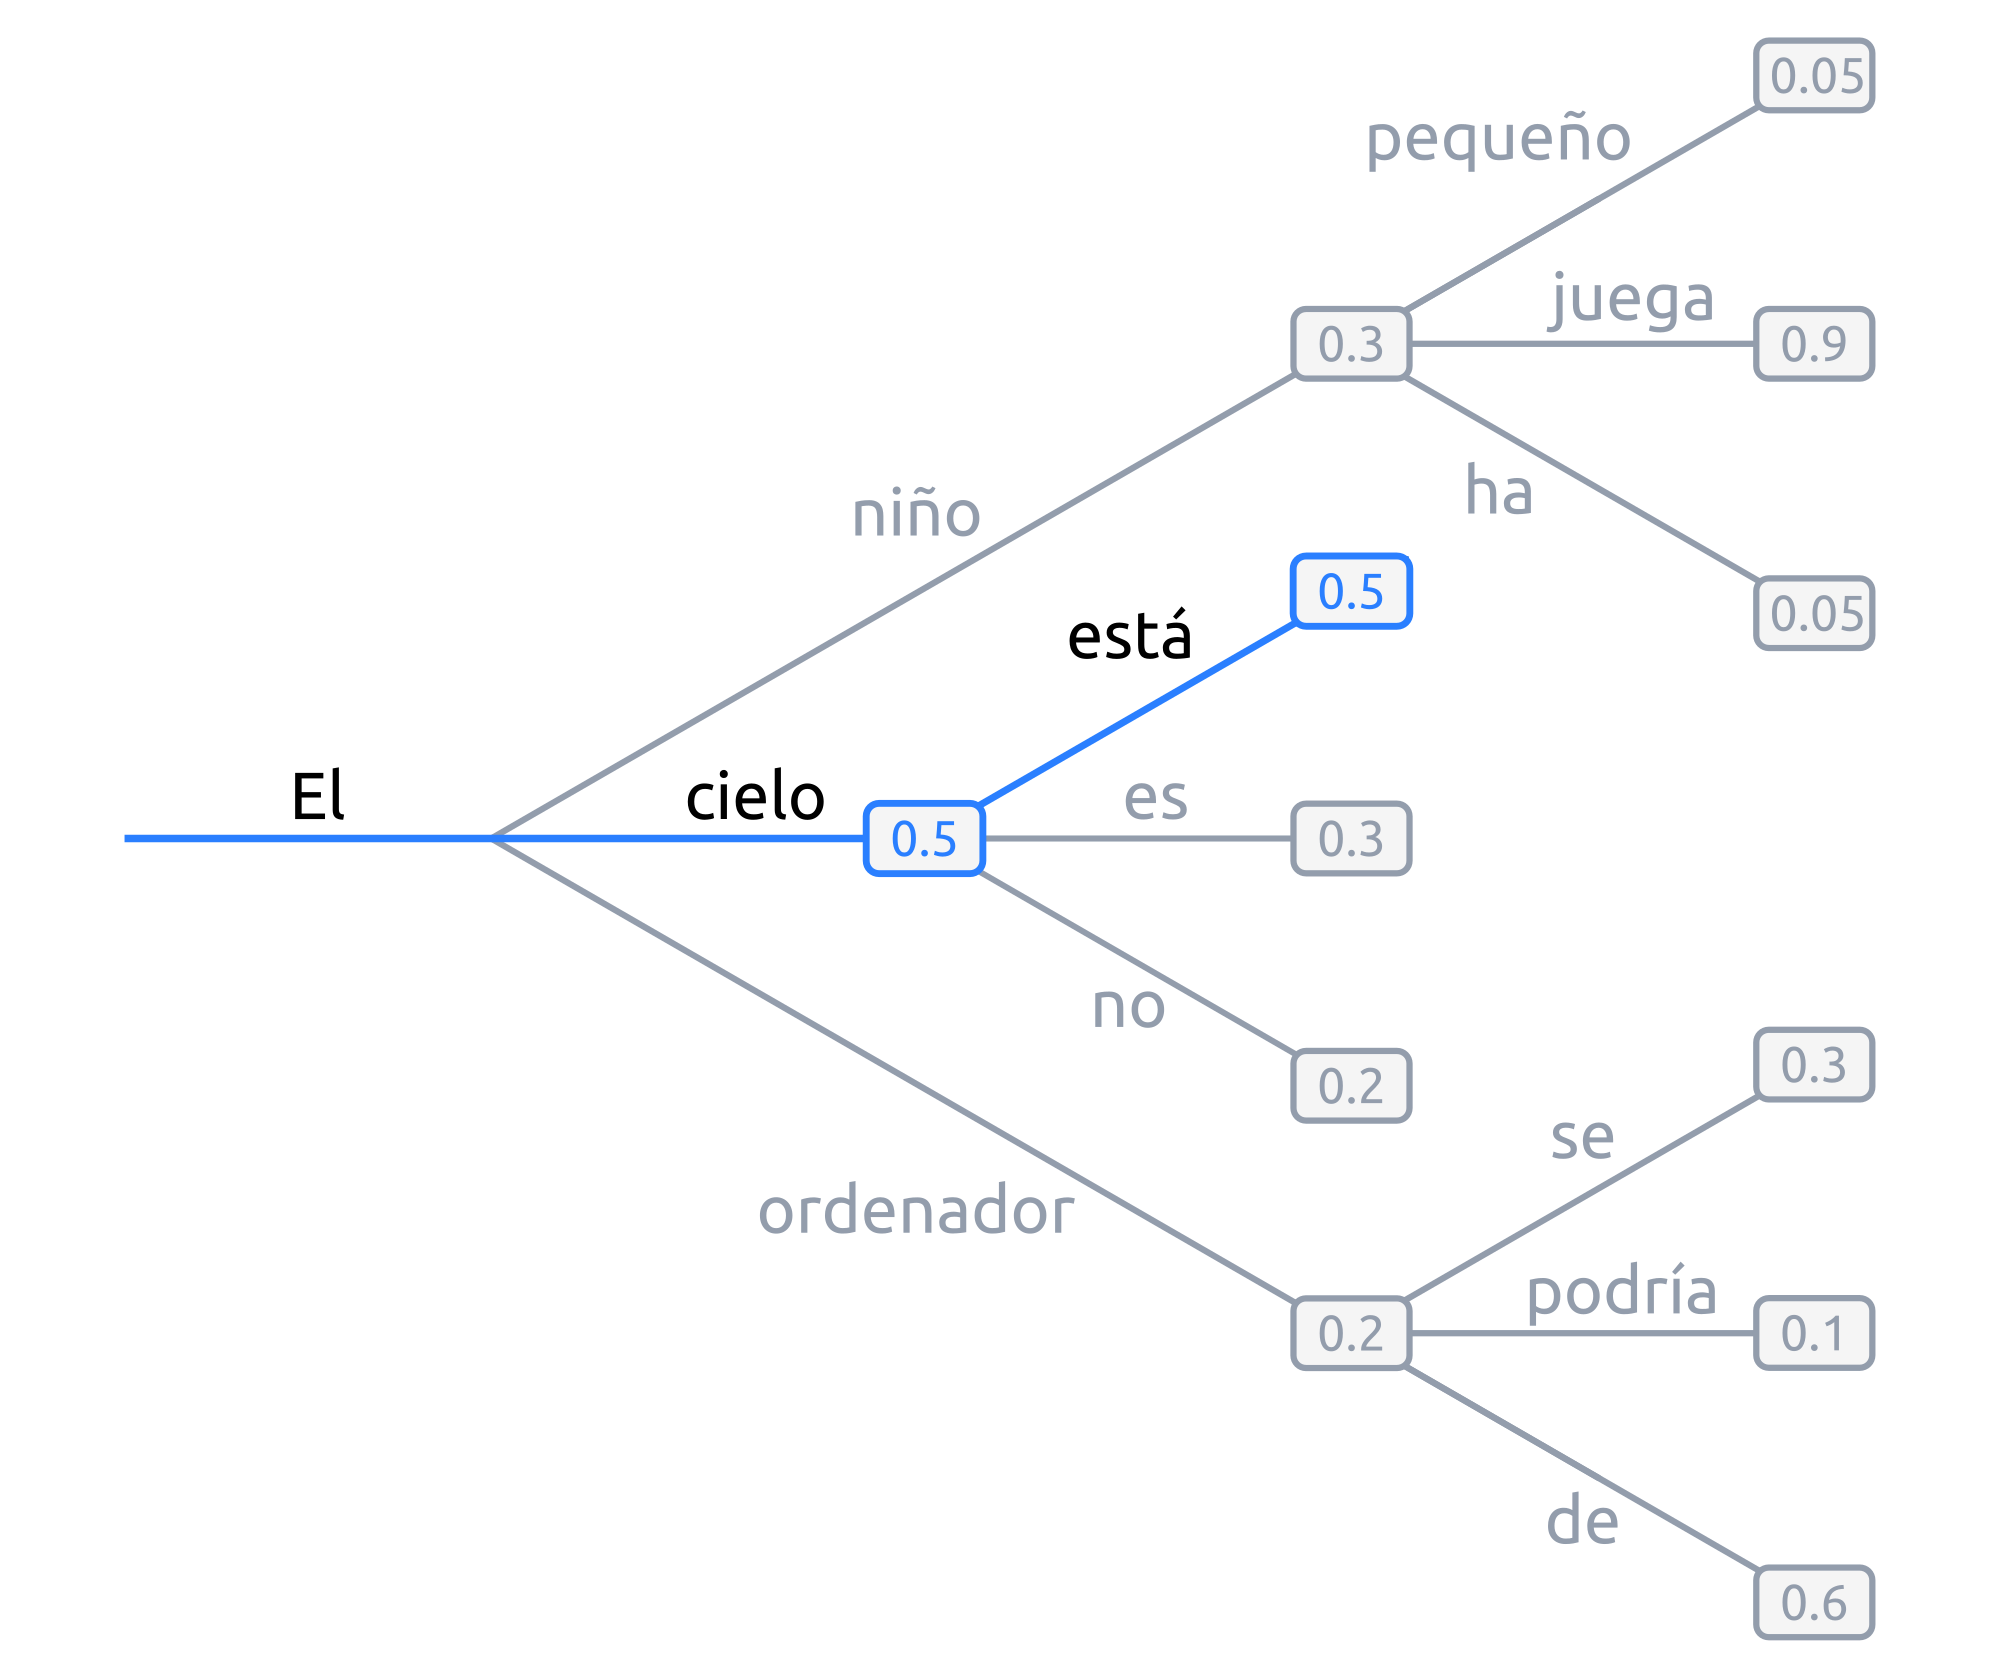
\includegraphics[width=0.7\textwidth]{greedy-search}
	\caption[Ejemplo de generación con búsqueda voraz.]{Ejemplo de búsqueda voraz: en cada paso, se toma la palabra con mayor probabilidad.}
\end{figure}


Por ejemplo, dada la palabra \texttt{``El''}, la siguiente palabra elegida sería \texttt{``cielo''}, por ser la palabra con mayor probabilidad (0.5), y a continuación \texttt{``está''} (0.5), y así sucesivamente.

Este tipo de generación tiene dos problemas principales:

\begin{itemize}
	\item [\textbullet] Los modelos, llegados a cierto punto, comienzan a repetir las mismas palabras una y otra vez. En realidad, esto es un problema que afecta a todos los modelos de generación, pero especialmente a los que emplean búsqueda voraz y \emph{beam search} \cite{vijayakumar16, shao17}.
	\item [\textbullet] Palabras con probabilidades altas pueden quedar enmascaradas tras otras con probabilidades bajas. Por ejemplo, en el anterior anterior ejemplo, la secuencia \texttt{``El niño juega''} nunca se dará, porque a pesar de que \texttt{``juega''} presenta una probabilidad muy alta (0.9), está precedida por \texttt{`niño''}, la cual no será escogida por tener una probabilidad baja (0.3).
\end{itemize}


\bigskip
\noindent
\textbf{\emph{Beam search}}

En este caso, durante el proceso de generación se consideran varios caminos simultáneamente, y finalmente se escoge aquel camino que presenta una mayor probabilidad conjunta. En la \hyperref[fig:beam-search]{siguiente figura} se ilustra un ejemplo con dos caminos (\texttt{num\_beams = 2}).

\begin{figure}[!h]
	\centering
	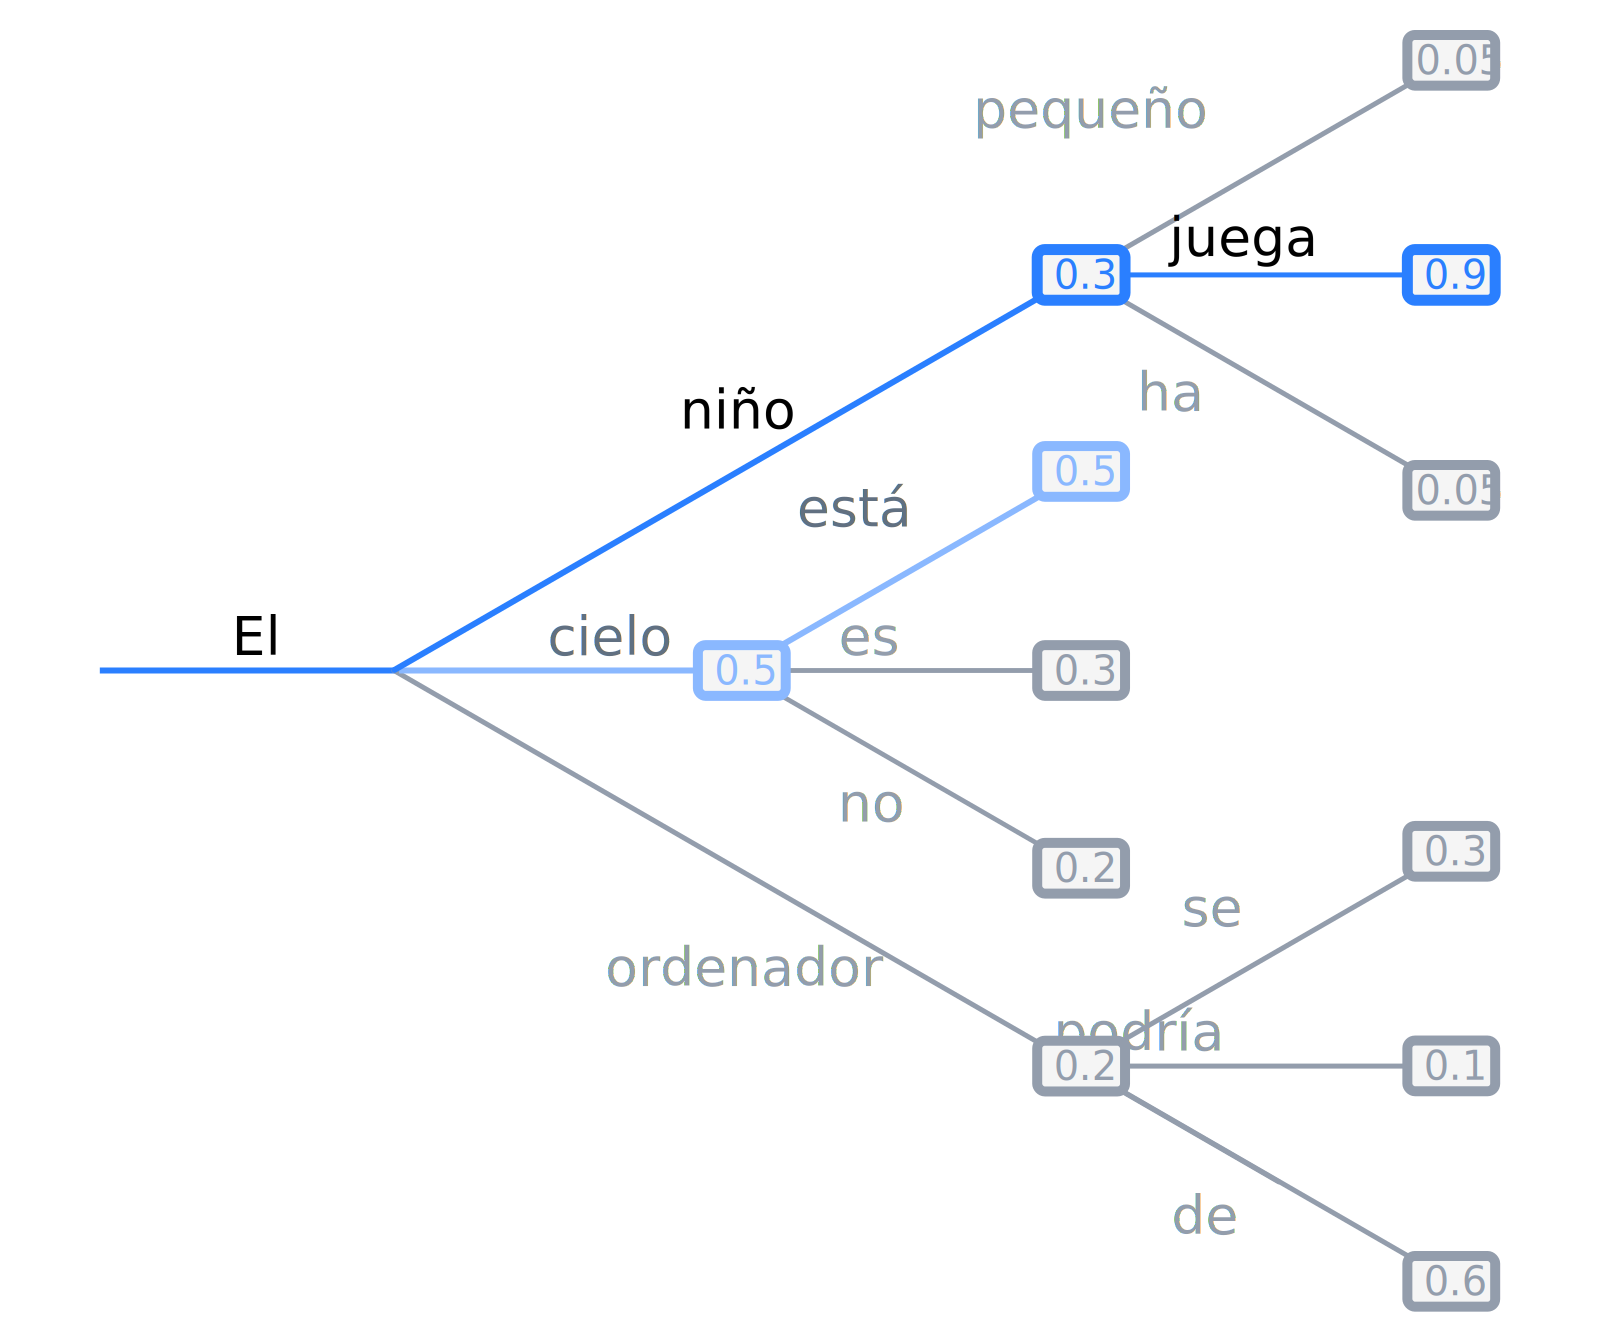
\includegraphics[width=0.7\textwidth]{beam-search}
	\caption[Ejemplo de generación con búsqueda \emph{beam-search}.]{Ejemplo de \emph{beam search} con \texttt{n\_beams = 2}. Durante la búsqueda, se consideran los dos caminos con mayor probabilidad conjunta.}
	\label{fig:beam-search}
\end{figure}

En este ejemplo vemos que, aunque \texttt{``cielo''} presenta mayor probabilidad que \texttt{``niño''}, la secuencia \texttt{``El niño juega''} tiene una mayor probabilidad conjunta ($0.3 \cdot 0.9 = 0.27$) que \texttt{``El cielo está''} ($0.5 \cdot 0.5  = 0.25$), y por tanto será la secuencia elegida.

Este tipo de búsqueda funciona muy bien en tareas en las que la longitud deseada de la secuencia generada se conoce de antemano, como es el caso de la generación de resúmenes, o la traducción automática \cite{murray18, yang18}.

Sin embargo, presenta dos problemas fundamentales:

\vspace*{-\baselineskip}
\begin{itemize}
	\item [\textbullet] De nuevo, aparece el problema de la repetición. Tanto en este caso, como en el de la búsqueda voraz, una estrategia común para evitar dicha repetición, consiste en establecer penalizaciones de \emph{n-gramas} repetidos. Por ejemplo, en el caso de que empleáramos una penalización de 6-gramas, la secuencia \texttt{``El niño juega en el parque''} solo podría aparecer una vez en el texto generado.

	\item [\textbullet] Como se razona en \cite{holtzman20}, el lenguaje humano no sigue una distribución de palabras con mayor probabilidad. Como vemos en la siguiente gráfica, extraída de dicho artículo, la estrategia de \emph{beam search} puede resultar poco espontánea, dando lugar a textos menos <<naturales>>:
	
	\begin{figure}[!h]
		\centering
		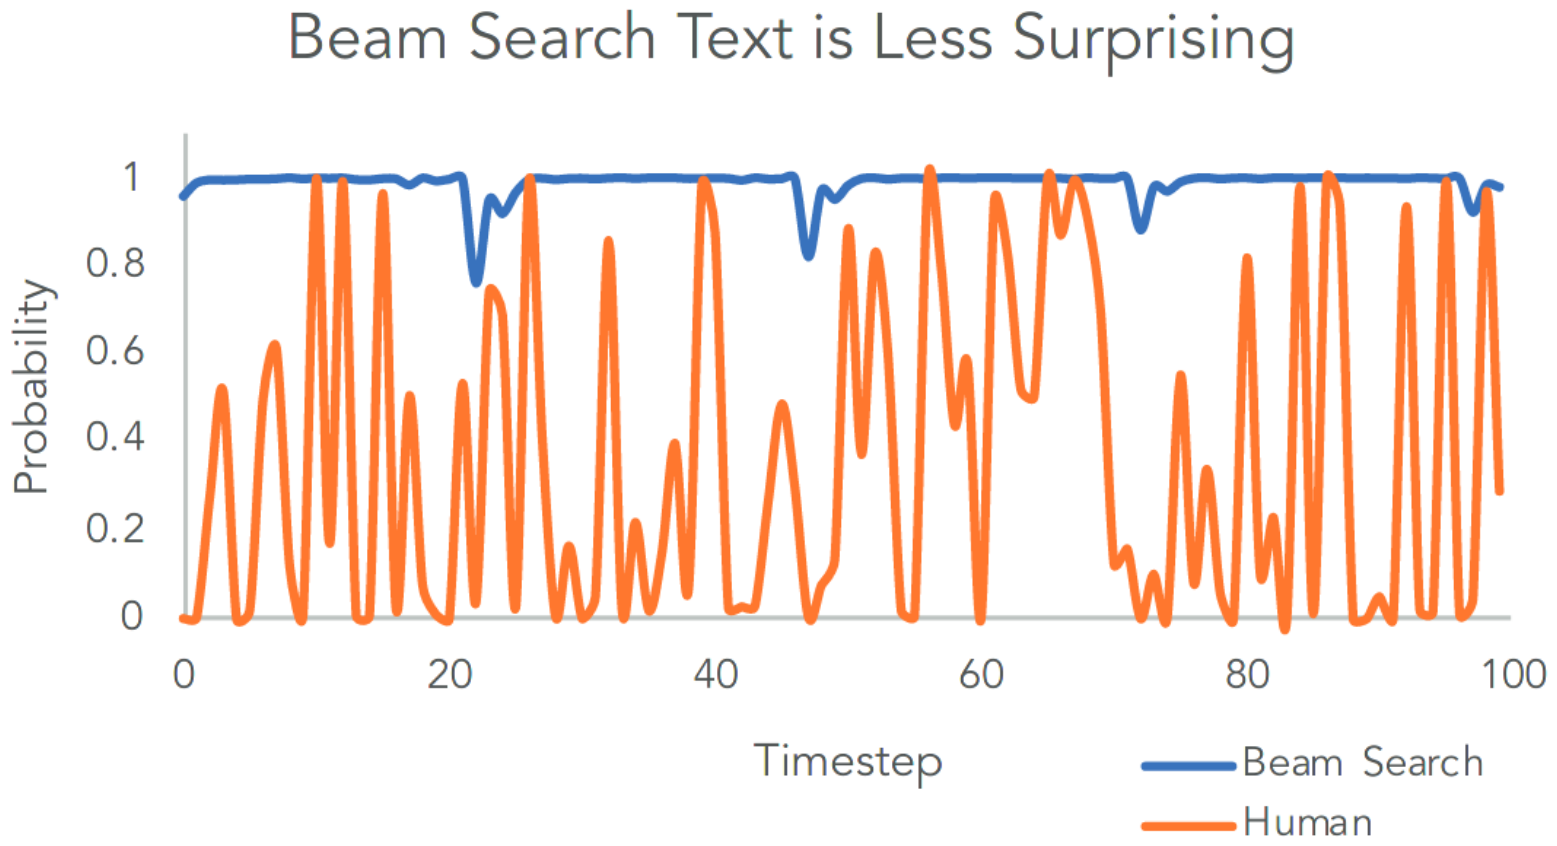
\includegraphics[width=0.7\textwidth]{beam-search-problem}
		\caption[Distribución de probabilidades en la generación.]{Distribución de probabilidades del lenguaje natural frente a la estrategia de \emph{beam search} \cite{holtzman20}.}
	\end{figure}
\end{itemize}


\bigskip
\noindent
\textbf{Muestreo}

Es su forma más básica, el muestreo simplemente consiste en escoger la siguiente palabra $w_i$ de manera aleatoria en función de la distribución de su probabilidad condicional, es decir:

\[ w_t \sim P(w_t | w_{1:t-1}) \]

De manera gráfica, siguiendo con el ejemplo anterior:

\begin{figure}[!h]
	\centering
	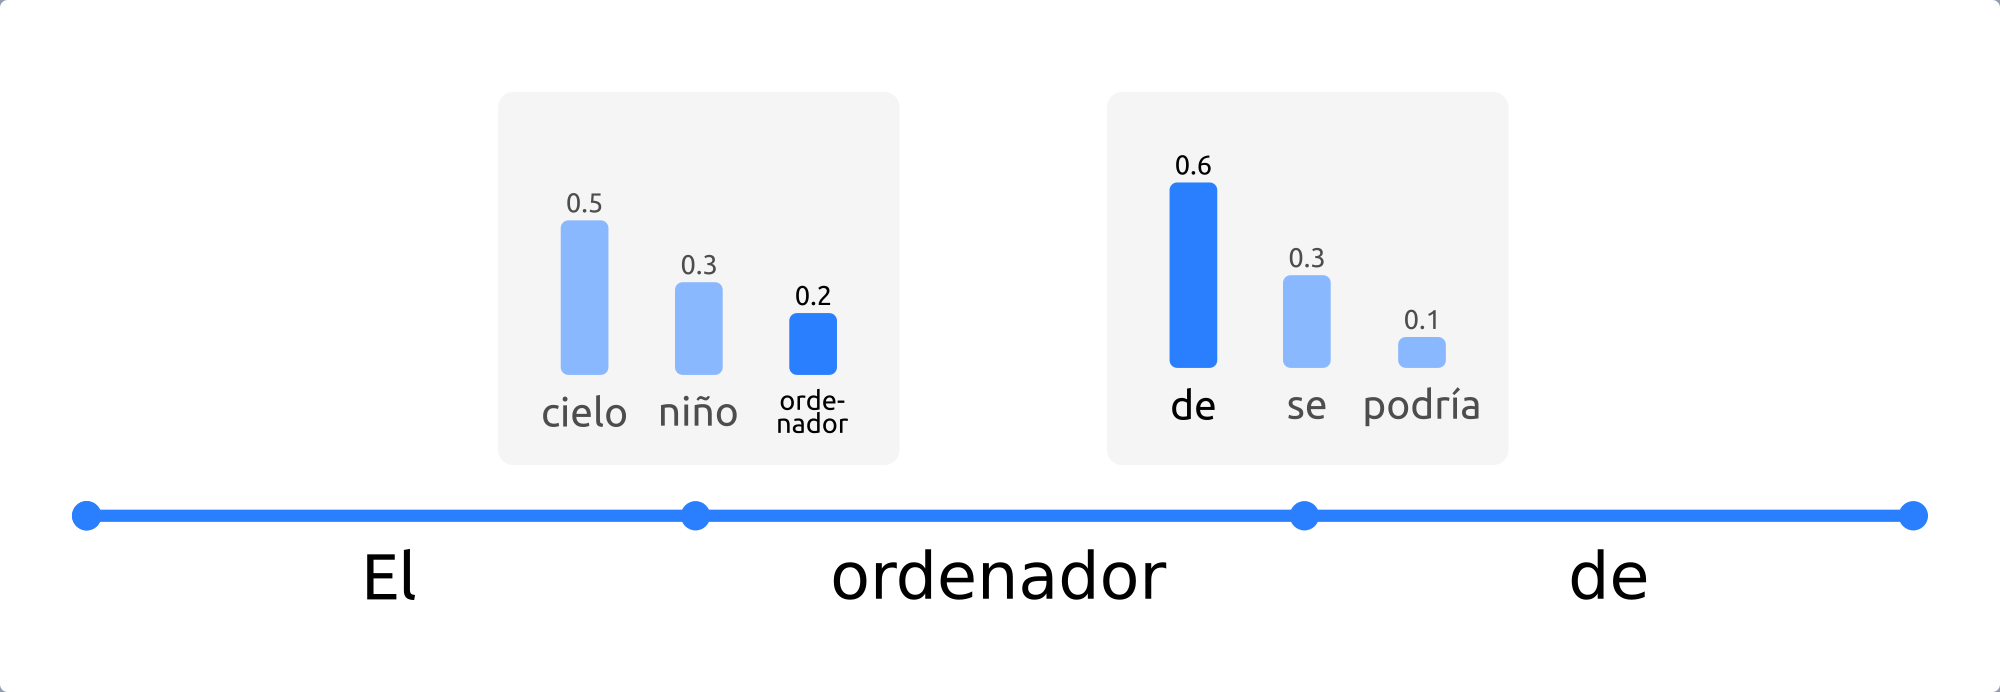
\includegraphics[width=0.8\textwidth]{sampling}
	\caption[Ejemplo de muestreo.]{Ejemplo de muestreo. En cada paso, se elige una palabra aleatoriamente en función de su probabilidad.}
	\label{fig:muestreo}
\end{figure}

Haciendo uso del muestreo, la generación deja de ser determinista, dando lugar a textos más espontáneos y naturales. Sin embargo, como se estudia en \cite{holtzman20}, esta espontaneidad es a menudo excesiva, dando lugar a textos poco coherentes.

Una solución a este problema consiste en hacer que la distribución $P(w_t|w_{1:t-1})$ sea más acusada, aumentando la verosimilitud (\emph{likelihood}) de palabras con alta probabilidad, y disminuyendo la verosimilitud de palabras con baja probabilidad. Esto se consigue disminuyendo un parámetro denominado \emph{temperatura}\footnote{\hspace{0.06cm}Por motivos de brevedad, no incluiremos una explicación detallada de este parámetro.}. De esta forma, el \hyperref[fig:muestreo]{ejemplo anterior} queda de la siguiente forma:

\begin{figure}[!h]
	\centering
	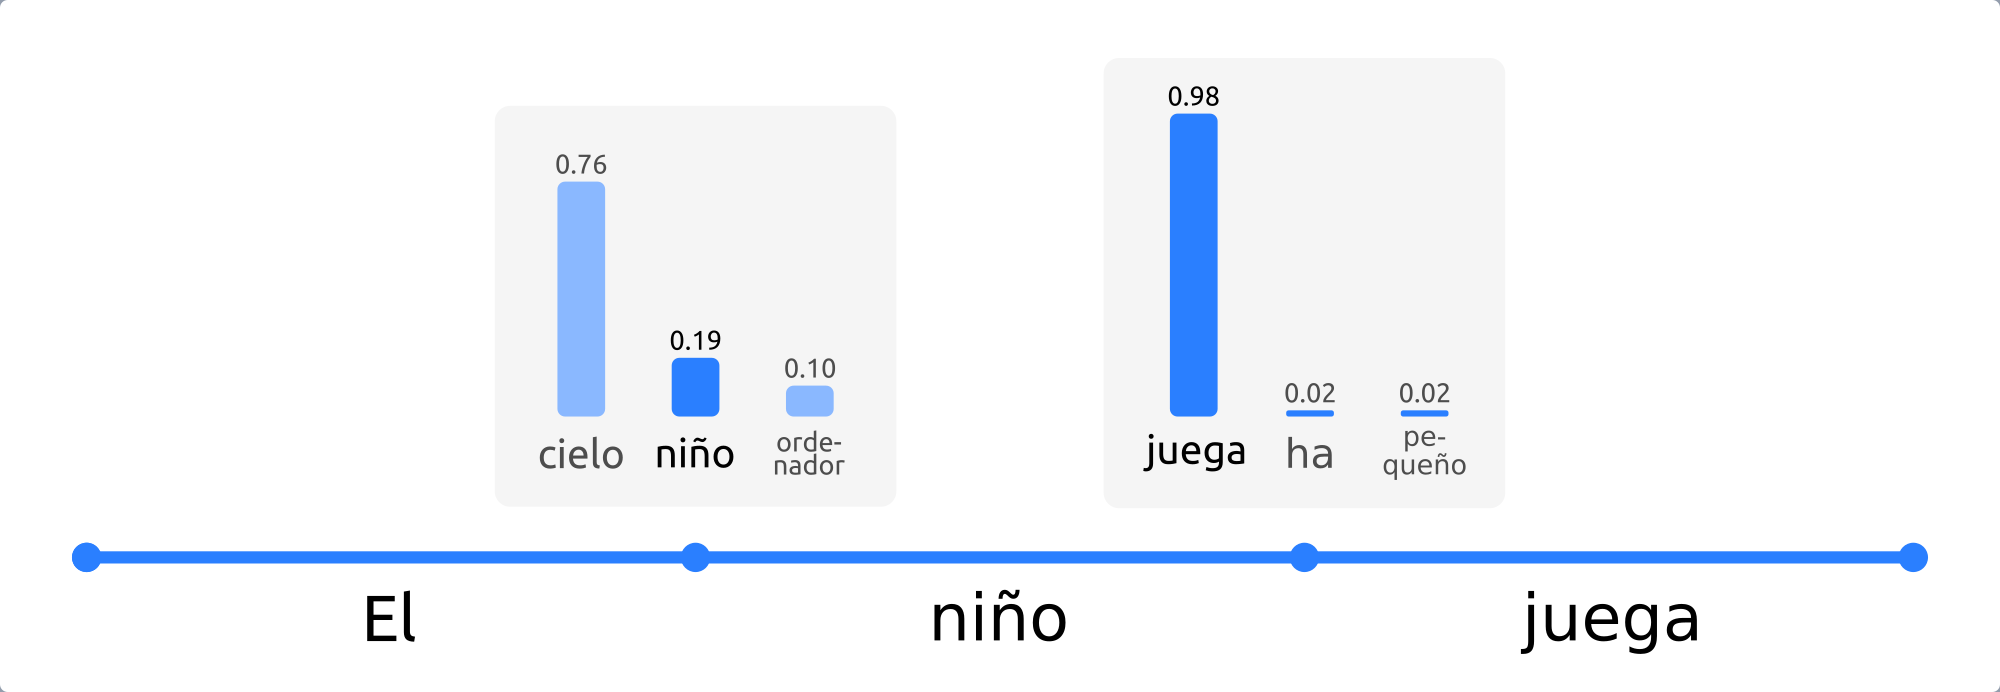
\includegraphics[width=0.8\textwidth]{sampling-temperature}
	\caption[Ejemplo de muestreo con temperatura.]{Al decrementar la temperatura, las diferencias en las  probabilidades se hacen más acusadas.}
\end{figure}

Con este ajuste de la temperatura, logramos reducir la aleatoriedad, pero seguimos manteniendo una orientación no determinista.

\newpage

\bigskip
\noindent
\textbf{Muestreo \emph{top-k}}

En ste tipo de muestreo, introducido en \cite{fan18}, en cada paso solo se consideran las \emph{k} palabras con mayor probabilidad (la probabilidad del resto de las palabras será 0).

\begin{figure}[!h]
	\centering
	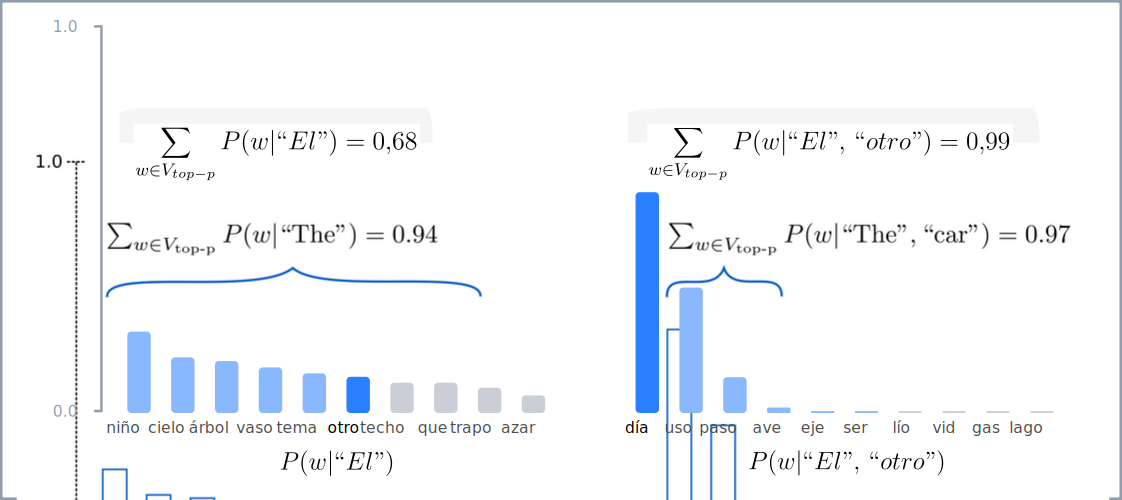
\includegraphics[width=\textwidth]{top-k}
	\caption[Ejemplo de muestreo \emph{top-k}.]{Ejemplo de muestreo \emph{top-k}. En cada paso, solo se consideran las 6 palabras con mayor probabilidad.}
	\label{fig:top-k}
\end{figure}

Tanto la búsqueda voraz como el muestreo visto anteriormente, se pueden como casos particulares del muestreo \emph{top-k}. Si establececemo $k = 1$, estaremos realizando una búsqueda voraz, y si establecemos $k = N$, donde $N$ es la longitud total del vocabulario, estaremos llevando a cabo un muestreo <<puro>>.

Este tipo de muestreo suele producir textos de mayor calidad en situaciones en las que el tamaño de secuencia no está prefijado. Sin embargo, presenta el problema de que el tamaño de \emph{k} se mantiene fijo a lo largo de la generación. Como consecuencia, en pasos en los que la diferencia de probabilidades sea menos acusada, como en el primer paso de la \autoref{top-k}, la espontaneidad del modelo será menor, y en pasos en los que ocurra lo contrario, el modelo será más propenso de escoger palabras que suenen menos naturales, como podría haber ocurrido en el segundo paso de la figura ya mencionada.


\bigskip
\noindent
\textbf{Muestreo \emph{top-p}}

Este tipo de muestreo, en vez de escoger entre un número prefijado de palabras, en cada paso considera el mínimo conjunto de palabras cuyas probabilidades acumuladas superan un cierto valor $p$ \cite{holtzman20}.

\begin{figure}[!h]
	\centering
	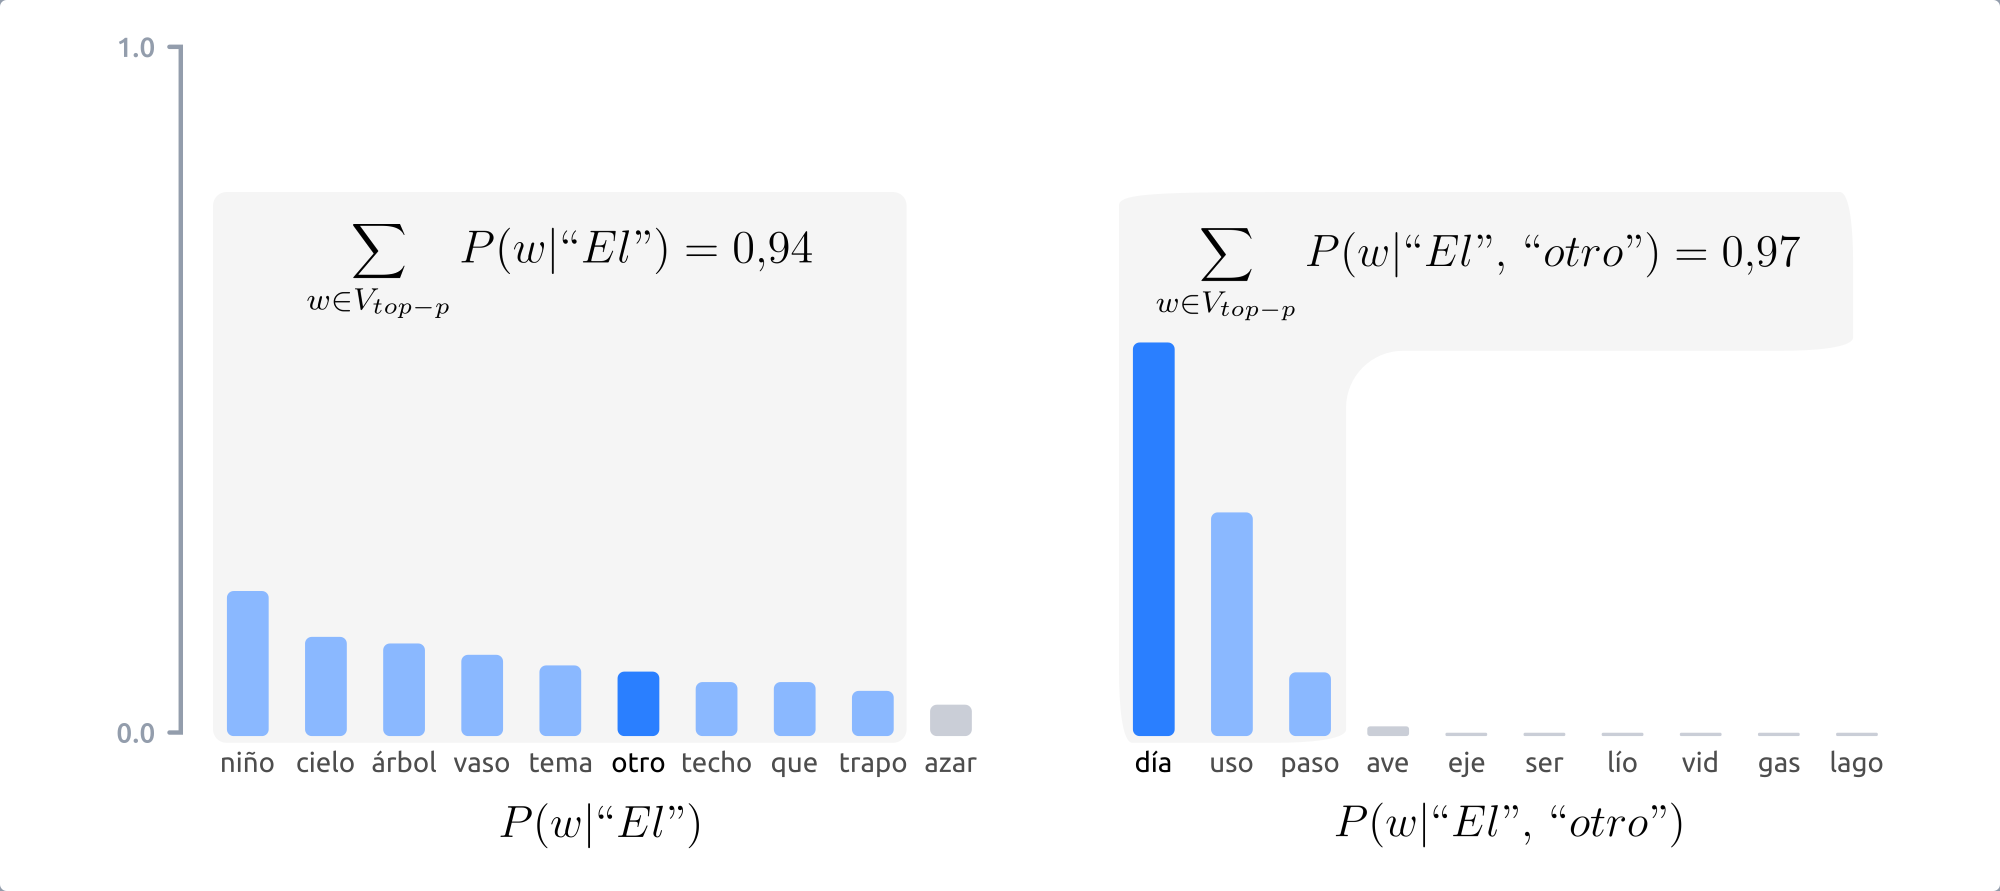
\includegraphics[width=\textwidth]{top-p}
	\caption[Ejemplo de muestreo \emph{top-p}.]{Con el muestreo \emph{top-p}, el número de palabras entre las cuales elegir en cada paso varía en función de las probabilidades de las palabras candidatas.}
	\label{fig:top-p}
\end{figure}

La \hyperref[top-p]{figura anterior} muestra como, con $p=0.9$, en el primer paso se consideran 9 palabras, mientras que en el segundo solo 3. De este modo, cuando la siguiente palabra a elegir es menos \emph{predecible}, el modelo puede considerar más candidatas, como en el primer paso del ejemplo mostrado y, en el caso contrario, el número de palabras candidatas se reduce.

Los resultados del muestreo \emph{top-k} u \emph{top-p} son, en la práctica, similares. De hecho, se pueden utilizar de manera conjunta, a fin de evitar la selección de palabras con probabilidades muy bajas, pero manteniendo cierta variación en el número de palabras consideradas.



\section{Post-procesado del texto} \label{sec:postprocesado}

Como veíamos en la \autoref{fig:proceso-resumen}, el resumen producido por el modelo T5, una vez decodificado, se encuentra todo en minúsculas. Por lo demás, el modelo parece hacer un buen trabajo a la hora de generar el texto en lo que a colocación de puntuación y espacios se refiere, luego la principal labor de esta etapa será poner mayúsculas allí donde sean necesarias, lo que en inglés se denomina \emph{truecasing} \cite{lita03}.

Las mayúsculas, tanto en inglés como español, se emplean principalmente en dos ocasiones:

\vspace*{-\baselineskip}
\begin{itemize}
	\item [\textbullet] Al inicio de cada frase. Como veíamos en la sección referente al \hyperref[sec:preprocesado]{pre-procesado} del texto, la separación de un texto en frases no es, por lo general, una tarea trivial. En este caso, podemos reutilizar lo aplicado en dicha etapa. Teniendo el resumen generado dividido en frases, podemos fácilmente poner la primera letra de cada una de ellas en mayúsculas.
	\item [\textbullet] En los nombres propios. En este aspecto, de nuevo vuelve a aparecer el problema del Reconocimiento de Entidades Nombradas (NER). De modo similar a como procedíamos en el pre-procesado, emplearemos un modelo estadístico que realiza la labor de \emph{truecasing}.
\end{itemize}

Tras esta etapa, el resumen está listo para ser entregado al usuario.